\documentclass{ieeeaccess}
\usepackage[utf8]{inputenc}
\usepackage[T1]{fontenc}
\usepackage{cite}

% ieeeaccess.cls upper-cases section titles with the TeX primitive
% \uppercase (see cls l.297), which processes the title byte-by-byte and
% corrupts multi-byte UTF-8 Turkish characters (İ, Ş, Ç, Ğ, ...). Since the
% section titles below are already written in correct Turkish uppercase, we
% neutralize the primitive so the titles are emitted verbatim.
\def\uppercase#1{#1}
\usepackage{amsmath,amssymb,amsfonts}
\usepackage{graphicx}
\usepackage{textcomp}
\usepackage[unicode]{hyperref}
\usepackage{booktabs}
\makeatletter
\AtBeginDocument{\DeclareMathVersion{bold}
\SetSymbolFont{operators}{bold}{T1}{times}{b}{n}
\SetSymbolFont{NewLetters}{bold}{T1}{times}{b}{it}
\SetMathAlphabet{\mathrm}{bold}{T1}{times}{b}{n}
\SetMathAlphabet{\mathit}{bold}{T1}{times}{b}{it}
\SetMathAlphabet{\mathbf}{bold}{T1}{times}{b}{n}
\SetMathAlphabet{\mathtt}{bold}{OT1}{pcr}{b}{n}
\SetSymbolFont{symbols}{bold}{OMS}{cmsy}{b}{n}
\renewcommand\boldmath{\@nomath\boldmath\mathversion{bold}}}
\makeatother

\def\BibTeX{{\rm B\kern-.05em{\sc i\kern-.025em b}\kern-.08em
    T\kern-.1667em\lower.7ex\hbox{E}\kern-.125emX}}

\begin{document}
\history{Sürüm tarihi: 25/05/2026}
\doi{}

\title{Communities and Crime Veri Seti Üzerinde İstatistiksel Veri Analizi}
\author{Serkan Eren\authorrefmark{1}}

\address[1]{Yapay Zekâ Yüksek Lisans Programı, Bilgisayar Mühendisliği Bölümü, Mühendislik Fakültesi, Gebze Teknik Üniversitesi, Kocaeli, Türkiye}

\tfootnote{Bu çalışma, Gebze Teknik Üniversitesi Yüksek Lisans Programı kapsamında verilen CSE 555: İstatistiksel Veri Analizi dersinin dönem projesi olarak yürütülmüştür.}

\markboth
{S.~Eren: Communities and Crime Veri Seti Üzerinde İstatistiksel Veri Analizi}
{S.~Eren: Communities and Crime Veri Seti Üzerinde İstatistiksel Veri Analizi}

\corresp{s.eren2018@gtu.edu.tr}

\begin{abstract}
Bu çalışma, UCI \emph{Communities and Crime} veri setinin yapısını keşifsel, istatistiksel ve boyut-indirgemeli analizler dizisiyle incelemektedir. Veri setinin 122 öngörücü özniteliği, etiketten bağımsız ve veri-güdümlü bir özellik seçim hattıyla önce kırk üç normalize sosyodemografik değişkene indirgenir: düşük kapsama sahip LEMAS öznitelikleri çıkarılır, kalan öngörücüler mutlak Pearson korelasyon uzaklığı ($d = 1 - |r|$, tam bağlantı) üzerinde aglomeratif hiyerarşik kümelemeyle gruplanır ve her kümeden bir temsilci tutulur. Sürekli hedef değişken \texttt{ViolentCrimesPerPop}, tertillere göre Düşük, Orta ve Yüksek suç sınıflarına ayrıştırılır. Boru hattı; özellik-başına kutu grafiği incelemesi ve Isolation Forest tabanlı çok-değişkenli aykırı değer temizliği, Pearson ve Spearman korelasyon analizi, z-skor normalizasyonu ile özellik-başına Fisher Uzaklığı, temel bileşen analizi (PCA) ile temel bileşen-başına Fisher Uzaklığı, doğrusal ayırma analizi (LDA), ve K-Means, DBSCAN, t-SNE ile Öz-Düzenleyici Harita (SOM) projeksiyonlarının karşılaştırmasını içerir. 2-B gömmelerde sınıf ayrılabilirliği silüet katsayısı ve 5-NN çapraz doğrulama doğruluğu ile nicel olarak raporlanmış; SOM organizasyonu nöron-başına sınıf-saflığı ısı haritasıyla özetlenmiştir. Analiz, aile-yapısı ve sosyoekonomik temsilcilerin (örn. \texttt{PctKids2Par}, \texttt{PctIlleg}, \texttt{PctPopUnderPov}) en güçlü tekil sınıf sinyalini taşıdığını, başat PCA bileşeninin bu ayırt edici içeriğin büyük kısmını miras aldığını ve LDA'nın PCA'ya göre daha sıkı sınıf-ayrılabilir bir 2-B gömme ürettiğini göstermektedir. Düşük ve Yüksek sınıfları arasında \texttt{PctKids2Par} üzerinde uygulanan Welch t-testi, $n=36$ ve $n=64$ için son derece anlamlı bir ortalama farkı ortaya koymaktadır.
\end{abstract}

\begin{keywords}
Communities and Crime, keşifsel veri analizi, hiyerarşik kümeleme, özellik seçimi, Fisher Uzaklığı, PCA, LDA, K-Means, DBSCAN, t-SNE, Öz-Düzenleyici Harita, hipotez testi.
\end{keywords}

\titlepgskip=-21pt
\maketitle

% ===================================================================
\section{GİRİŞ}
\label{sec:introduction}
\PARstart{U}{CI} Makine Öğrenmesi Deposundan elde edilen \emph{Communities and Crime} veri seti \cite{uciccrime}, Amerika Birleşik Devletleri'nde topluluk düzeyinde şiddet suçunun sosyodemografik modellenmesi için yaygın olarak kullanılan bir kıyaslama veri setidir. Veri seti; 1990 ABD Nüfus Sayımı, 1990 ABD Kolluk Kuvvetleri Yönetim ve İdari İstatistikleri (LEMAS) anketi ve 1995 FBI Birleşik Suç Raporlarından (UCR) elde edilen bilgileri birleştirir \cite{redmondbaveja} ve $128$ öznitelikle tanımlanan $1\,994$ topluluk içermektedir. Her öngörücü öznitelik, farklı nüfus büyüklüğüne sahip topluluklar arasında karşılaştırmaların anlamlı olabilmesi için veri seti yazarları tarafından $[0,1]$ aralığına normalize edilmiştir.

Bu çalışmanın amacı rekabetçi bir tahmin modeli inşa etmek değil, gerçek, karışık kaliteli bu veri setinin istatistiksel yapısını birbirini tamamlayan keşifsel, boyut-indirgemeli ve çıkarımsal analizler dizisiyle karakterize etmek ve her yöntemin veri hakkında ortaya koyduğunu yorumlamaktır. Merkezî bir metodolojik tercih, çalışılan özellik kümesinin sübjektif elle seçimini, tamamen veri-güdümlü ve etiket-kör bir boyut indirgeme prosedürüyle değiştirmektir. Somut olarak, düşük kapsamlı öznitelikler önce dışlanır; ardından geri kalan öngörücüler mutlak Pearson korelasyon uzaklığı üzerinde aglomeratif hiyerarşik kümeleme ile gruplanır ve her kümeden bir temsilci tutulur. Bu prosedür; demografi, etnik kompozisyon, kentleşme, gelir ve konut maliyeti, eğitim, istihdam, yoksulluk, aile yapısı, göç, konut kalitesi ve ikamet hareketliliği gibi orijinal veri setinin her kavramsal bloğunu kapsayan, küme-içi ikili korelasyonu alttan sınırlı tutan $43$ sosyodemografik özelliklik bir çalışma kümesi üretir. Seçim mekanizması Bölüm~\ref{sec:dataset}'de tanımlanmıştır. Problemi çok-sınıflı bir çerçeveye oturtmak için, sürekli hedef değişken \texttt{ViolentCrimesPerPop} tertillere göre eşit-frekanslı üç sınıfa ayrıştırılır: \emph{Düşük}, \emph{Orta} ve \emph{Yüksek}.

Makalenin geri kalanı şu şekilde organize edilmiştir. Bölüm~\ref{sec:dataset} veri setini, eksik veri filtresini ve dendrogram tabanlı özellik seçimini açıklar. Bölüm~\ref{sec:boxplot} özellik dağılımlarını inceler ve çok-değişkenli aykırı değer temizliği uygular. Bölüm~\ref{sec:corr} özellikler arasındaki ve sınıf etiketiyle korelasyon yapısını çözümler; Bölüm~\ref{sec:fisher} özellik-başına ayırt ediciliği Fisher Uzaklığı ile niceler. Bölüm~\ref{sec:pca}--\ref{sec:pcscatter} temel-bileşen yapısını ve düşük-boyutlu sınıf projeksiyonlarını inceler; Bölüm~\ref{sec:lda} bunları denetimli bir doğrusal ayırma gömmesiyle karşılaştırır. Bölüm~\ref{sec:cluster} denetimsiz küme yapısını K-Means, DBSCAN, t-SNE ve Öz-Düzenleyici Harita ile araştırır; Bölüm~\ref{sec:hypothesis} başat öngörücünün anlamlılığını sınar. Bölüm~\ref{sec:conclusion} temel bulguları özetler.

% ===================================================================
\section{VERİ SETİ VE ÖZELLİK SEÇİMİ}
\label{sec:dataset}
Communities and Crime veri seti \cite{uciccrime}; $128$ sütunla tanımlanan $1\,994$ topluluk içerir: beş tane öngörücü olmayan tanımlayıcı (\texttt{state}, \texttt{county}, \texttt{community}, \texttt{communityname}, \texttt{fold}), $122$ öngörücü aday ve hedef öznitelik \texttt{ViolentCrimesPerPop}. Tüm öngörücü değişkenler, veri seti yazarları tarafından $\pm 3$ standart sapmanın ötesindeki değerleri kırpan denetimsiz eşit-aralıklı binning yöntemiyle önceden $[0,1]$ aralığına normalize edilmiştir; bu normalizasyon değişken-içi dağılım şeklini korur ancak değişkenler arası göreli büyüklükleri korumaz. Sürekli yanıt \texttt{ViolentCrimesPerPop}, tertillere göre eşit-frekanslı üç sınıfa ayrıştırılır: \emph{Düşük}, \emph{Orta} ve \emph{Yüksek}; bu, temizlik öncesi $679 / 662 / 653$ örnek dağılımını verir. Tüm işlemler Python~3.10 ortamında \texttt{NumPy}, \texttt{pandas}, \texttt{scikit-learn} \cite{pedregosa}, \texttt{scipy}, \texttt{seaborn} ve \texttt{MiniSom} \cite{minisom} kütüphaneleri kullanılarak yürütülmüştür.

\subsection{TANIMLAYICI SÜTUNLARIN VE EKSİK VERİNİN FİLTRELENMESİ}
\label{ssec:miss}
Beş tanımlayıcı sütun ilk adımda düşürülmüştür. Veri seti ardından LEMAS polis-gücü anketinden türetilmiş, $22$ değişkenden oluşan bitişik bir blok içerir (örn. \texttt{LemasSwornFT}, \texttt{PolicPerPop}, \texttt{RacialMatchCommPol}); bu blok $1\,994$ topluluğun $1\,675$'i için, yani örneklemin $\%84$'ü için eksiktir. Böylesine derin bir boşluğu doldurmak, sonraki kovaryans-tabanlı yöntemlerde (PCA, LDA, Fisher Uzaklığı) ciddi yapay varyans enjekte ederek tüm analizi kirletecektir; bu nedenle bu $22$ sütun tamamen kaldırılmıştır. Geriye kalan $100$ öngörücüde sütun başına en fazla $\%0.05$ eksiklik bulunmakta olup sütun-medyanı ile doldurulmuştur.

\subsection{KORELASYON UZAKLIĞI ÜZERİNDE HİYERARŞİK KÜMELEMEYLE ÖZELLİK SEÇİMİ}
\label{ssec:fselect}
Hayatta kalan $100$ öngörücü hâlâ ağır kavramsal redundancy taşımaktadır: \texttt{medIncome}, \texttt{medFamInc}, \texttt{perCapInc}, \texttt{whitePerCap} ve mülk-sahip-oturan konut değer çeyrekleri \texttt{OwnOcc\{Low,Med,Hi\}Quart}'ın tümü aynı altta yatan yapıyı (topluluk varlığı) ölçer ve ikili $|r| > 0{,}85$ değerlerinde korelasyonludur. Elle düzenlenen bir çalışma kümesi kaçınılmaz olarak analistin önceki beklentilerini yansıtır; biz bu seçimi, özelliklerin ikili-korelasyon geometrisindeki aglomeratif hiyerarşik kümelemesine \cite{hastie} dayanan tamamen etiket-kör bir prosedürle değiştiririz. Sınıf etiketi seçim sürecinde hiçbir şekilde danışılmadığı için, sonraki denetimli analizler (Fisher Uzaklığı, LDA, K-NN ayrılabilirliği) seçimden kaynaklanan veri sızıntısından arınmış kalır.

Aynı bilgiyi taşıyan iki özellik, korelasyonlarının işaretinden bağımsız olarak redundant kabul edilmelidir: \texttt{racePctWhite} ve \texttt{racepctblack} $r \approx -0{,}85$ civarında korelasyonludur fakat tek bir etnik-kompozisyon eksenini kodlamaktadır. Bu nedenle, mutlak değerli Pearson korelasyon uzaklığını kullanırız:
\begin{equation}
d_{ij} \;=\; 1 - |r_{ij}|, \qquad d_{ij}\in[0,1],
\label{eq:corrdist}
\end{equation}
bu tanım, hem mükemmel pozitif hem mükemmel negatif korelasyonlu çiftleri $d=0$'a, istatistiksel olarak bağımsız çiftleri ise $d=1$'e götürür. $100$ öngörücü üzerindeki sıkıştırılmış ikili uzaklık matrisi, \emph{tam bağlantı} (complete linkage) ile aglomeratif kümelemeye verilir. Tam bağlantı, iki kümeyi yalnızca aralarındaki \emph{en büyük} ikili uzaklık eşiği aşmadığında birleştirir; bu, ortaya çıkan her kümede ikili korelasyonun en az $1 - d_{\mathrm{th}}$ ile alttan sınırlanmasını garanti eder. Ortalama ve tekil bağlantı bu garantiyi sağlamaz ve sıkı ile gevşek korelasyonlu üyeleri karıştıran kümeler üretir.

$d_{\mathrm{th}}\in\{0{,}20, 0{,}25, \ldots, 0{,}60\}$ aralığında bir eşik taraması sırasıyla $57$ ile $29$ arasında küme verir. $d_{\mathrm{th}} = 0{,}35$ çalışma noktası --- küme-içi korelasyon tabanı $|r|\geq 0{,}65$'e karşılık gelen --- benimsenmiştir. Bu seçim tam olarak $43$ küme üretir; bu, dört büyük belirgin redundancy bloğunun (gelir/varlık, aile yapısı, yoksunluk ve yakın göç payları) tek gruplara konsolide olduğu, ama kavramsal olarak ayrı boyutların (örn. göç yakınlık oranları ile nüfus içindeki göçmen payı, ya da iki-ebeveynli haneler ile hiç evlenmemiş anneler) ayrı kaldığı en küçük küme sayısıdır. Şekil~\ref{fig:dendrogram} elde edilen dendrogramı, kesim çizgisi ve renk-kodlu kümelerle birlikte göstermektedir.

\begin{figure*}[!t]
\centering
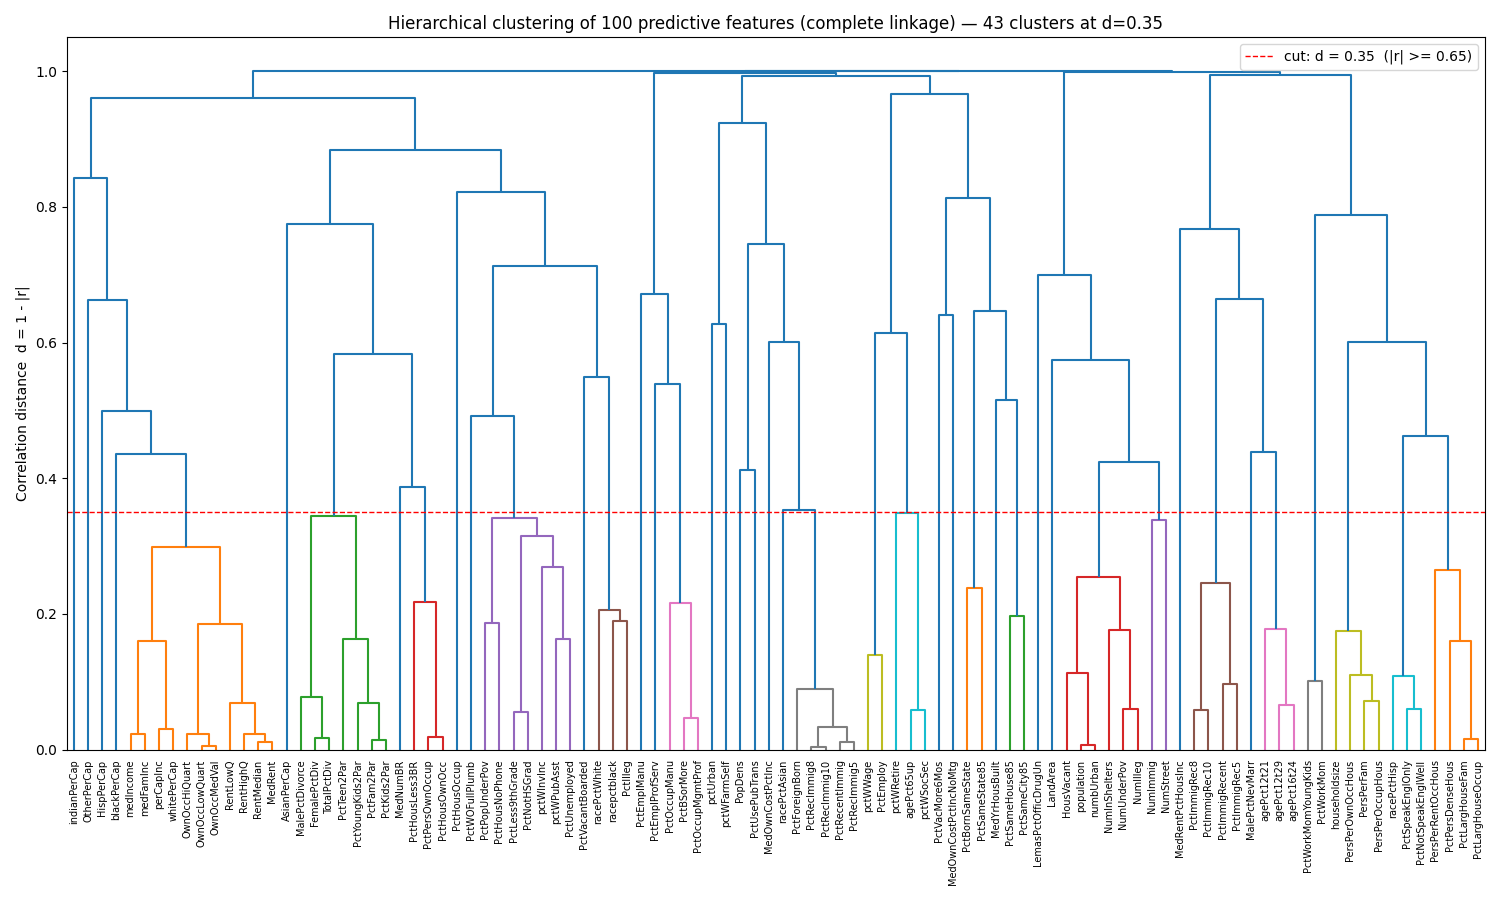
\includegraphics[width=\textwidth]{feature_dendrogram.png}
\caption{$100$ öngörücü adayının mutlak Pearson korelasyon uzaklığı $d = 1 - |r|$ üzerinde tam bağlantı ile aglomeratif hiyerarşik kümelemesi. $d=0{,}35$ değerindeki yatay kırmızı çizgi, $43$ küme üreten ve küme-içi korelasyon tabanını $|r|\geq 0{,}65$ ile sınırlayan kesimdir. Kesim altında herhangi bir alt-ağaca katılmayan (yani $d \approx 1$'e ulaşan dikey yapraklar) singleton kümeler, kavramsal olarak benzersiz bilgi taşıyan özelliklere karşılık gelir.}
\label{fig:dendrogram}
\end{figure*}

\subsection{KÜME TEMSİLCİSİNİN SEÇİMİ}
\label{ssec:rep}
$43$ kümenin her birinden tam olarak bir temsilci tutulur. Singleton kümelerde temsilci, kümenin tek üyesidir ($24$ singleton). Çok-üyeli her küme için varsayılan kural, \emph{merkez (centroid)} özelliği almaktır; yani diğer üyelere ortalama ikili korelasyon uzaklığı en düşük olan üye, kümeyi kendi başına en iyi özetleyen özelliktir. $19$ çok-üyeli kümeden $7$'sinde merkez, kriminoloji ve sosyal-bilimler literatüründe yaygın kullanılan bir değişkenle örtüşmekte olduğundan olduğu gibi tutulmuştur. Diğer $12$ çok-üyeli kümede ise, yorumlanabilirlik-güdümlü bir geçersiz kılma uygulanarak yakın-eşdeğer merkez yerine kanonik literatür değişkeni tercih edilmiştir (örn. gelir-ve-varlık kümesinde merkez \texttt{RentHighQ} yerine \texttt{medIncome}'a geçilmiştir; çünkü medyan gelir, ilgili literatürde topluluk-varlığının standart vekil değişkenidir). Tüm geçersiz kılmalar, yer aldıkları kümenin içinde kalır; bu nedenle küme-içi korelasyon garantisi korunur. Çok-üyeli kümeler ve nihai temsilcileri Tablo~\ref{tab:clusters}'de listelenmiştir.

\begin{table*}[!t]
\caption{$d_{\mathrm{th}}=0{,}35$'te elde edilen $19$ çok-üyeli küme, üyeleri ve sonraki analizler için tutulan temsilcileri. ``$\star$'' algoritmik merkezi işaretler; seçilen temsilci \textbf{koyu} olarak gösterilmiştir. Singleton kümeler ($24$ özellik) Tablo~\ref{tab:features}'de listelenmiştir.}
\label{tab:clusters}
\centering
\footnotesize
\begin{tabular}{cclp{7.6cm}}
\toprule
Küme & Boyut & Tema & Üyeler (merkez $\star$, temsilci \textbf{koyu}) \\
\midrule
 1 & 11 & Gelir / varlık                & \textbf{medIncome}, medFamInc, perCapInc, whitePerCap, OwnOcc\{Low,Med,Hi\}Quart, Rent\{Low,Med\}Q, RentHighQ$^\star$, MedRent \\
 6 &  7 & Aile yapısı                   & MalePctDivorce, FemalePctDiv, TotalPctDiv, PctFam2Par$^\star$, \textbf{PctKids2Par}, PctYoungKids2Par, PctTeen2Par \\
 7 &  3 & Konut sahipliği               & PctPersOwnOccup$^\star$, PctHousLess3BR, \textbf{PctHousOwnOcc} \\
10 &  7 & Yoksunluk                     & pctWInvInc, pctWPubAsst, \textbf{PctPopUnderPov}, PctLess9thGrade, PctNotHSGrad$^\star$, PctUnemployed, PctHousNoPhone \\
12 &  3 & Irk / evlilik-dışı doğum      & racepctblack, racePctWhite, \textbf{PctIlleg}$^\star$ \\
15 &  3 & Eğitim / meslek               & \textbf{PctBSorMore}, PctOccupManu, PctOccupMgmtProf$^\star$ \\
22 &  5 & Göç payı                      & PctRecentImmig, PctRecImmig5, PctRecImmig8$^\star$, PctRecImmig10, \textbf{PctForeignBorn} \\
25 &  2 & İstihdam                      & pctWWage$^\star$, \textbf{PctEmploy} \\
26 &  3 & Yaşlı / emeklilik             & \textbf{agePct65up}$^\star$, pctWSocSec, pctWRetire \\
29 &  2 & Eyalet-düzeyi ikamet          & \textbf{PctBornSameState}$^\star$, PctSameState85 \\
30 &  2 & Yerel ikamet                  & \textbf{PctSameHouse85}$^\star$, PctSameCity85 \\
32 &  6 & Nüfusa ölçekli sayımlar       & \textbf{population}$^\star$, numbUrban, NumUnderPov, NumIlleg, HousVacant, NumInShelters \\
33 &  2 & Nüfusa ölçekli sayımlar       & \textbf{NumImmig}$^\star$, NumStreet \\
36 &  4 & Göç yakınlığı                 & PctImmigRecent, PctImmigRec5, \textbf{PctImmigRec8}$^\star$, PctImmigRec10 \\
37 &  3 & Genç yaş yapısı               & agePct12t21, \textbf{agePct12t29}, agePct16t24$^\star$ \\
40 &  2 & Çalışan annelik               & PctWorkMomYoungKids$^\star$, \textbf{PctWorkMom} \\
41 &  4 & Hane büyüklüğü                & \textbf{householdsize}, PersPerFam, PersPerOccupHous$^\star$, PersPerOwnOccHous \\
42 &  3 & Hispanik / dil                & \textbf{racePctHisp}, PctSpeakEnglOnly, PctNotSpeakEnglWell$^\star$ \\
43 &  4 & Kalabalık barınma             & PctLargHouseFam, PctLargHouseOccup$^\star$, PersPerRentOccHous, \textbf{PctPersDenseHous} \\
\bottomrule
\end{tabular}
\end{table*}

\subsection{NİHAİ ÇALIŞMA KÜMESİ}
\label{ssec:final}
Bölüm~\ref{ssec:miss}--\ref{ssec:rep}'deki prosedür, $43$ özellikten oluşan deterministik bir çalışma kümesi üretir --- $24$'ü singleton kümelerden, $19$'u çok-üyeli kümelerden gelmek üzere --- Tablo~\ref{tab:features}'de kavramsal bloklara göre listelenmiştir. Tutulan her özellik, veride redundant olmayan bir varyasyon eksenini temsil eder; daha kesin ifadeyle, hiçbir iki tutulan özellik seçilen korelasyon tabanı altında aynı hiyerarşik-kümeleme kümesinin içinde yer almaz. Kümeler-arası korelasyonlar bu prosedürle elbette sınırlanmaz: örneğin 12.\ kümenin temsilcisi \texttt{PctIlleg} ile 6.\ kümenin temsilcisi \texttt{PctKids2Par}, hâlâ $|r|\approx 0{,}87$ ile korelasyonludur; çünkü dendrogram bu iki özelliği, kavramsal olarak yakın fakat birbirinden ayrılabilir iki ``yoğunlaşmış dezavantaj'' ekseni olarak ifşa eder. Bu küme-arası kalan korelasyon, veri setine ilişkin başlı başına bir gözlemdir ve Bölüm~\ref{sec:corr} ile \ref{sec:pca}'de tekrar ele alınmıştır. Aynı $43$-özellik çalışma kümesi, sonraki tüm analizlerde kullanılır.

\begin{table}[!t]
\caption{Kavramsal bloklara göre gruplandırılmış $43$ tutulan özellik. Tüm değişkenler veri seti yazarları tarafından zaten $[0,1]$ aralığına normalize edilmiştir.}
\label{tab:features}
\centering
\footnotesize
\begin{tabular}{p{1.7cm}p{5.9cm}}
\toprule
Blok & Özellikler \\
\midrule
Demografi       & \texttt{population}, \texttt{householdsize}, \texttt{agePct12t29}, \texttt{agePct65up}, \texttt{racePctAsian}, \texttt{racePctHisp} \\
Kentleşme       & \texttt{pctUrban}, \texttt{PopDens}, \texttt{PctUsePubTrans}, \texttt{LandArea} \\
Gelir / varlık  & \texttt{medIncome}, \texttt{blackPerCap}, \texttt{HispPerCap}, \texttt{AsianPerCap}, \texttt{indianPerCap}, \texttt{OtherPerCap} \\
Konut maliyeti  & \texttt{MedOwnCostPctInc}, \texttt{MedOwnCostPctIncNoMtg}, \texttt{MedRentPctHousInc} \\
Eğitim          & \texttt{PctBSorMore} \\
İstihdam        & \texttt{PctEmploy}, \texttt{PctEmplProfServ}, \texttt{PctEmplManu}, \texttt{pctWFarmSelf} \\
Yoksulluk       & \texttt{PctPopUnderPov} \\
Aile            & \texttt{PctKids2Par}, \texttt{PctIlleg}, \texttt{MalePctNevMarr}, \texttt{PctWorkMom} \\
Göç             & \texttt{NumImmig}, \texttt{PctForeignBorn}, \texttt{PctImmigRec8} \\
Konut kalitesi  & \texttt{PctHousOwnOcc}, \texttt{MedNumBR}, \texttt{PctVacantBoarded}, \texttt{PctHousOccup}, \texttt{PctVacMore6Mos}, \texttt{MedYrHousBuilt}, \texttt{PctWOFullPlumb}, \texttt{PctPersDenseHous} \\
Hareketlilik    & \texttt{PctBornSameState}, \texttt{PctSameHouse85} \\
Polislik        & \texttt{LemasPctOfficDrugUn} \\
\bottomrule
\end{tabular}
\end{table}

% ===================================================================
\section{ÖZELLİK DAĞILIMLARI VE AYKIRI DEĞERLERİN TEMİZLENMESİ}
\label{sec:boxplot}
Şekil~\ref{fig:box_before}, seçilen $43$ değişkenin aykırı değer temizliği öncesi özellik-başına kutu grafiklerini, okunabilirlik için iki panele bölünmüş ve kavramsal bloklara göre etiketlenmiş biçimde sunmaktadır. Üç dağılım örüntüsü göze çarpar. İlk olarak, birçok özellik güçlü biçimde sağa çarpıktır ve uzun bir üst kuyruğa sahiptir --- en belirgin olarak \texttt{population}, \texttt{PopDens}, \texttt{LandArea}, \texttt{NumImmig}, \texttt{PctIlleg} ve \texttt{PctVacantBoarded}; bu kuyruklar, demografik veya sosyoekonomik olarak uç noktada bulunan küçük bir topluluk kümesini yansıtır (çok büyük ya da yoğun şehirler, çok yüksek göçmen sayıları veya yoğunlaşmış yoksunluk). İkincisi, koruyucu aile ve konut değişkenleri (\texttt{PctKids2Par}, \texttt{PctHousOwnOcc}, \texttt{PctEmploy}) \emph{sola} çarpıktır; uzun bir alt kuyrukları dezavantajlı topluluklardan oluşur. Üçüncüsü, \texttt{pctUrban} belirgin biçimde iki-modludur (bimodal): kutusu neredeyse tüm $[0,1]$ aralığını kaplar; çünkü topluluklar ağırlıklı olarak ya tamamen kentsel ($\approx 1$) ya da tamamen kırsaldır ($\approx 0$); bu, sonraki bölümlerdeki projeksiyonları yorumlarken hatırlanması gereken bir özelliktir. Buna karşılık \texttt{agePct12t29}, \texttt{agePct65up} ve kişi-başı gelir değişkenleri medyanları etrafında sıkıca toplanmıştır.

\begin{figure}[!t]
\centering
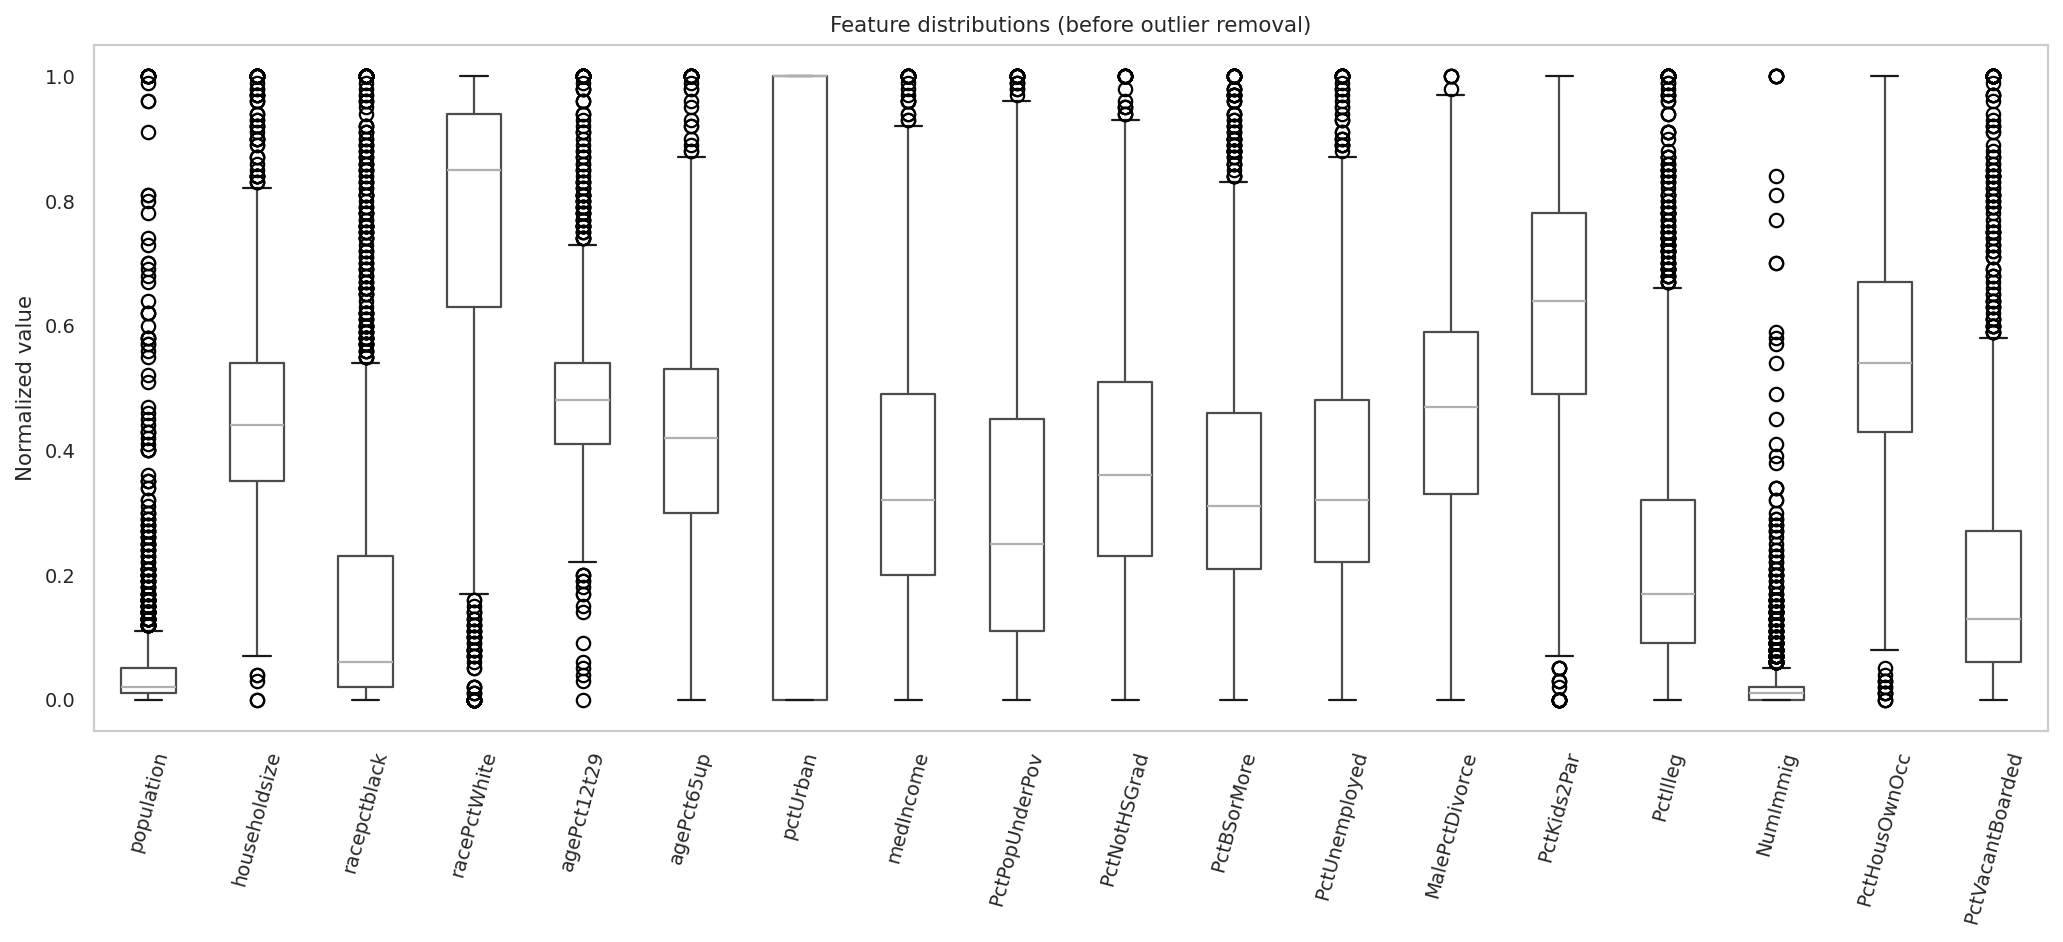
\includegraphics[width=\columnwidth]{boxplot_before.png}
\caption{Aykırı değer temizliği öncesinde seçilen $43$ özelliğin, kavramsal bloklara göre gruplandırılmış kutu grafikleri. Birçok sosyoekonomik değişken uzun üst kuyruklu sağa-çarpıklık gösterir, aile/konut koruyucu değişkenleri sola-çarpıktır ve \texttt{pctUrban} iki-modludur.}
\label{fig:box_before}
\end{figure}

\textbf{Neden çok-değişkenli bir detektör.} Univariate IQR reddi gibi bir özellik-başına filtre, \emph{herhangi bir} tek boyutta uç değer taşıyan örneği atar. Bu, buradaki veri için iki kez uygunsuzdur. Kavramsal olarak, birkaç sınıf-ayırt edici özellik (\texttt{PctPopUnderPov}, \texttt{PctIlleg}, \texttt{PctVacantBoarded}) doğası gereği neredeyse yalnızca Yüksek-suç topluluklarından oluşan ağır üst kuyruklar taşır; dolayısıyla marjinal kırpma, tam da analizin betimlemeye çalıştığı sınıfı boşaltır. İstatistiksel olarak, bir satırın işaretlenme olasılığı özellik sayısıyla hızla artar; çünkü bir satır, $43$ marjinalden \emph{en az birinde} eşiği aştığı anda reddedilir --- bu, boyutun lanetinin doğrudan bir tezahürüdür. Tablo~\ref{tab:outlier} her iki etkiyi de niceler: $k=3$ çarpanlı özellik-başına IQR kuralı $730$ satırı (verinin $\%36{,}6$'sı) atar ve Yüksek-suç sınıfını yarıdan fazla çökertir ($653 \rightarrow 295$, $-\%54{,}8$); bu da Bölüm~\ref{sec:fisher}--\ref{sec:lda}'daki denetimli analizleri anlamsız kılardı.

\begin{table}[!t]
\caption{$43$-özellik çalışma kümesinde aykırı değer temizleme karşılaştırması. Özellik-başına IQR kuralı yalnızca reddedilen bir taban olarak gösterilmiştir; fiilen kullanılan yöntem çok-değişkenli Isolation Forest'tır.}
\label{tab:outlier}
\centering
\small
\begin{tabular}{lccc}
\toprule
 & Öncesi & IQR ($k=3$) & Isolation Forest \\
\midrule
Tutulan satır        & $1\,994$ & $1\,264$ & $1\,894$ \\
Atılan satır         & ---      & $730\ (\%36{,}6)$ & $100\ (\%5{,}0)$ \\
\midrule
\emph{Düşük}         & $679$ & $524\ (-\%22{,}8)$ & $660\ (-\%2{,}8)$ \\
\emph{Orta}          & $662$ & $445\ (-\%32{,}8)$ & $649\ (-\%2{,}0)$ \\
\emph{Yüksek}        & $653$ & $295\ (-\%54{,}8)$ & $585\ (-\%10{,}4)$ \\
\bottomrule
\end{tabular}
\end{table}

Bu nedenle nihai boru hattı, \texttt{scikit-learn} \cite{pedregosa} kütüphanesinin çok-değişkenli \emph{Isolation Forest} \cite{liu2008isolation} yöntemini $200$ ağaç ve $\%5$ kirlilik (contamination) oranıyla kullanır. Detektör, her örneği özellik uzayının özyinelemeli rastgele bölünmesiyle yalıtır; yalıtılması olağandışı biçimde az sayıda rastgele bölme gerektiren bir örnek, $43$-boyutlu uzayın seyrek bir bölgesinde yer alır ve \emph{birleşik} (joint) bir anomali olarak işaretlenir. Kirlilik $=0{,}05$ ile filtre $100$ satırı ($\%5{,}0$) atar ve geriye sınıf dağılımı \emph{Düşük}: $660$, \emph{Orta}: $649$, \emph{Yüksek}: $585$ olan $1\,894$ topluluk bırakır (Tablo~\ref{tab:outlier}). Dikkat çekici olarak, Yüksek-sınıf daralması $43$-özellik kümesinde ($-\%10{,}4$), daha küçük bir $18$-özellik kümesine kıyasla (ön denemelerde $-\%11{,}6$) \emph{daha hafiftir}: ek boyutlar, detektöre meşru biçimde uç noktada bulunan Yüksek-suç topluluklarını, aynı anda birçok eksende gerçekten anomali olan topluluklardan ayırt etmek için daha fazla kanıt sağlar.

\begin{figure}[!t]
\centering
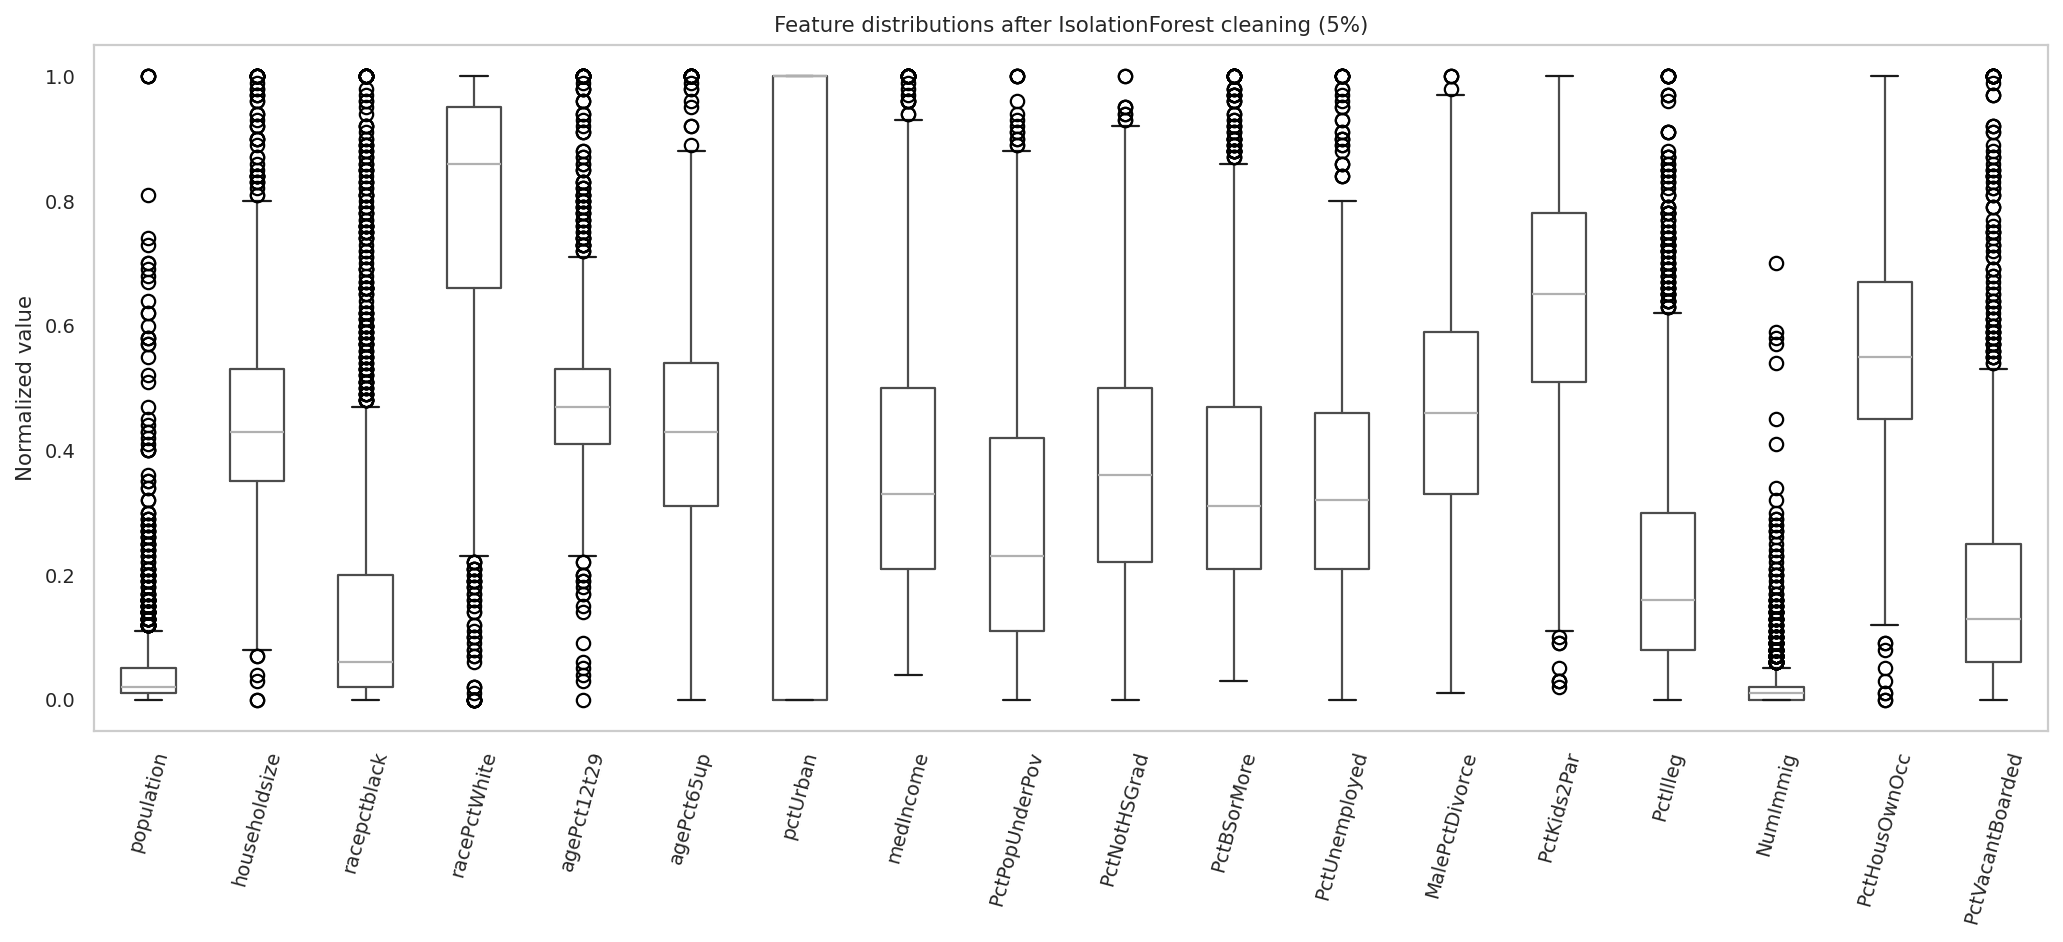
\includegraphics[width=\columnwidth]{boxplot_after.png}
\caption{Isolation Forest temizliği (kirlilik $=0{,}05$) sonrası kutu grafikleri. Her dağılımın ana gövdesi korunur, ancak marjinal aykırı değer noktaları (bıyıkların ötesindeki daireler) hâlâ görünürdür --- detektörün özellik-başına uç değerleri değil birleşik anomalileri kaldırdığının doğrudan görsel kanıtı.}
\label{fig:box_after}
\end{figure}

İnce ama önemli bir doğrulama Şekil~\ref{fig:box_after}'da görülebilir: birçok marjinal aykırı değer noktası (bıyıkların ötesindeki daireler) temizlik sonrasında \emph{korunmaktadır}. Özellik-başına bir IQR kuralı, yapısı gereği bıyıkların ötesinde hiç nokta bırakmayan kutu grafikleri üretirdi; bu noktaların burada varlığını sürdürmesi, Isolation Forest'ın bireysel bir eksende yalnızca uç olan değil, \emph{birleşik} $43$-boyutlu dağılımda anomali olan örnekleri hedeflediğini gösterir. Her özellik dağılımının niteliksel şekli --- çarpıklık, medyan ve çeyrekler-arası açıklık --- korunmuştur ve sonraki tüm analizler bu temizlenmiş $1\,894$ topluluk veri setini kullanır.

\section{KORELASYON YAPISI}
\label{sec:corr}
$43$ özellik ile ordinal kodlanmış sınıf etiketi arasındaki tam Pearson korelasyon matrisi Şekil~\ref{fig:corrheat}'da gösterilmektedir. $44$ satırla hücre-başına sayısal etiketler okunamaz olacağından bunlar çıkarılmış ve Tablo~\ref{tab:features}'deki kavramsal-blok sınırları siyah ayraçlar olarak çizilmiştir; bu durumda yalnızca renk alanı makro-yapıyı okunur kılar. Bölüm~\ref{sec:dataset}'in dendrogramının açığa çıkardığı aynı iki zıt süper-blok, burada korelasyon uzayında yeniden belirir. Bir \emph{avantaj} süper-bloğu --- medyan gelir ve kişi-başı gelir değişkenleri, eğitim (\texttt{PctBSorMore}), istihdam (\texttt{PctEmploy}), aile istikrarı (\texttt{PctKids2Par}) ve konut sahipliği (\texttt{PctHousOwnOcc}, \texttt{MedNumBR}) --- kendi içinde pozitif korelasyonludur. Bir \emph{dezavantaj} süper-bloğu --- yoksulluk (\texttt{PctPopUnderPov}), evlilik-dışı doğum (\texttt{PctIlleg}), aşırı kalabalıklaşma (\texttt{PctPersDenseHous}) ve konut çürümesi (\texttt{PctVacantBoarded}) --- benzer biçimde kendi içinde pozitif korelasyonludur. İki süper-blok birbiriyle güçlü biçimde negatif korelasyonludur; bu, makalenin geri kalanının tekrar tekrar geri kazandığı, iyi bilinen sosyoekonomik ``avantaj--dezavantaj'' gradyanıdır.

\begin{figure}[!t]
\centering
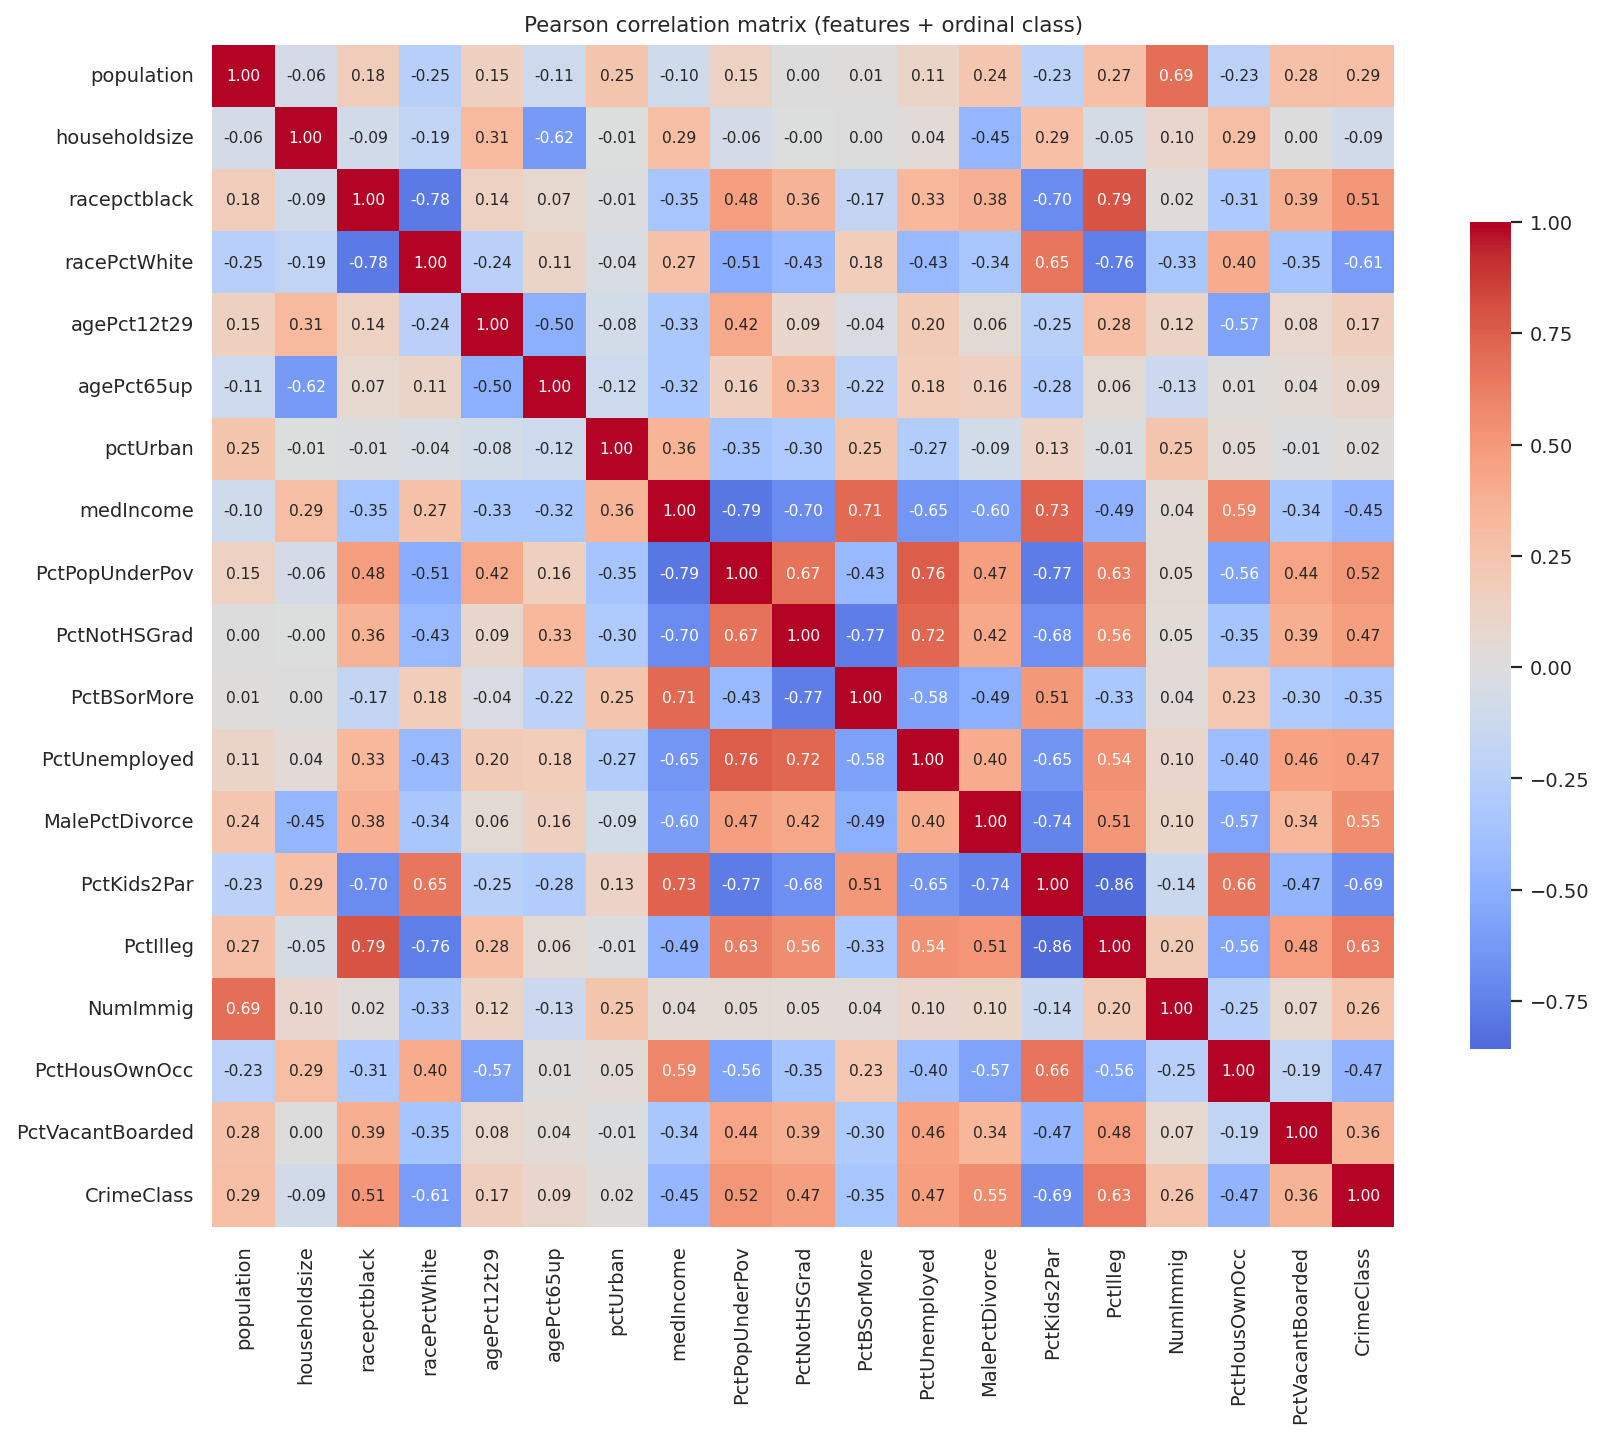
\includegraphics[width=\columnwidth]{correlation_heatmap.png}
\caption{$43$ özellik ile ordinal kodlanmış suç sınıfının Pearson korelasyon matrisi. Okunabilirlik için sayısal etiketler çıkarılmıştır; siyah çizgiler Tablo~\ref{tab:features}'deki kavramsal-blok sınırlarını işaretler. Zıt sıcak/soğuk bloklar, avantaj--dezavantaj sosyoekonomik gradyanıdır.}
\label{fig:corrheat}
\end{figure}

\begin{figure}[!t]
\centering
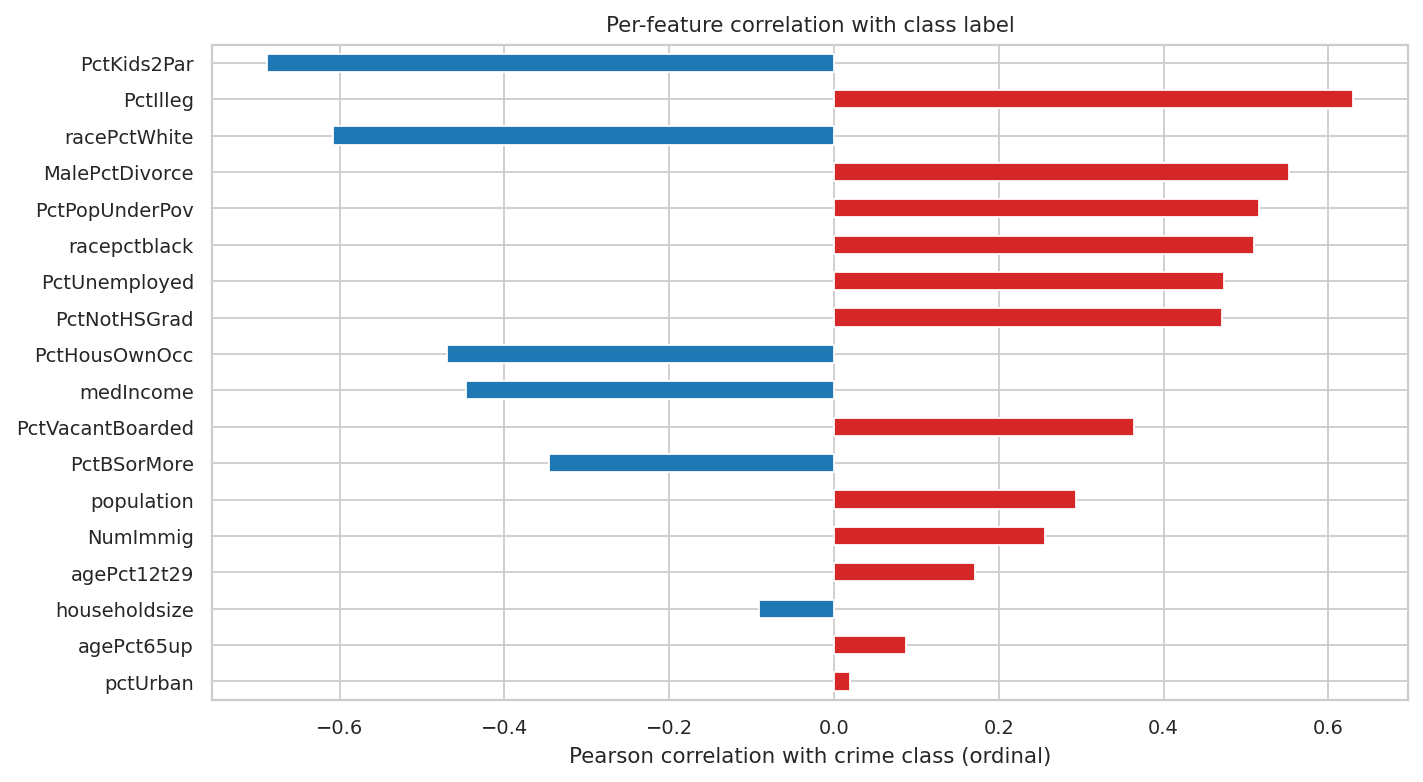
\includegraphics[width=\columnwidth]{feature_class_correlation.png}
\caption{$43$ özelliğin tamamının suç sınıfı (ordinal) ile özellik-başına Pearson korelasyonu, sıralanmış halde. Kırmızı çubuklar yüksek suç düzeyleriyle pozitif korelasyonu, mavi çubuklar negatif (koruyucu) korelasyonu gösterir.}
\label{fig:classcorr}
\end{figure}

Şekil~\ref{fig:classcorr}, $43$ özelliğin tamamını suç sınıfı (ordinal) ile korelasyonlarına göre sıralar. En güçlü tekil korelasyonlar \texttt{PctKids2Par} ($-0{,}69$), \texttt{PctIlleg} ($+0{,}62$), \texttt{PctPopUnderPov} ($+0{,}52$), \texttt{PctPersDenseHous} ($+0{,}47$), \texttt{PctHousOwnOcc} ($-0{,}46$), \texttt{medIncome} ($-0{,}45$) ve \texttt{PctVacantBoarded} ($+0{,}38$)'dir. İşaretler, topluluk düzeyinde suçun sosyal-düzensizlik açıklamasıyla tutarlıdır \cite{shawmckay}, \cite{sampson}: aile istikrarı, gelir, eğitim ve istikrarlı mülk-sahibi-oturan konut koruyucudur; buna karşılık yoksulluk, aile parçalanması ve konut çürümesi daha yüksek şiddet suçuyla birlikte görülür. İki gözlem veri-güdümlü $43$-özellik kümesine özgüdür. İlki, \texttt{PctPersDenseHous} (oda başına birden fazla kişi barındıran konutta yaşayan nüfus oranı) dördüncü en güçlü tekil korelasyon olarak belirir; bu aşırı kalabalıklaşma sinyali yoksulluktan kavramsal olarak ayrıdır ve daha küçük, elle seçilmiş bir kümede gözden kaçması kolay olurdu; ancak kümeleme boru hattı onu kendi bloğunun temsilcisi olarak tutar. İkincisi, konut-kalitesi bloğu rastlantısal değil kolektif olarak öngörücüdür: \texttt{PctHousOwnOcc}, \texttt{PctVacantBoarded}, \texttt{PctHousOccup} ve \texttt{MedNumBR}'nin tümü ilk on içinde yer alır; bu, konut stokunun fiziksel durumunun topluluk suçunu, kanonik gelir ve aile değişkenleri kadar yakından izlediğini gösterir. Diğer uçta, demografik ve coğrafi değişkenler --- \texttt{pctUrban}, \texttt{LandArea}, \texttt{agePct65up}, \texttt{householdsize}, \texttt{MedYrHousBuilt} ve etnisiteye-özgü kişi-başı gelir değişkenleri --- esasen hiçbir tekil sınıf sinyali taşımaz.

Sınıf etiketi aralık-ölçekli bir değişken yerine \emph{ordinal} bir tertil olduğundan, özellik--sınıf ilişkisi için Spearman sıra korelasyonu da hesaplanmıştır. Spearman büyüklükleri tipik olarak biraz daha büyüktür (örn. \texttt{PctKids2Par} $-0{,}70$, \texttt{PctIlleg} $+0{,}69$, \texttt{PctPopUnderPov} $+0{,}57$). En belirgin kayma \texttt{PctPersDenseHous}'dur; $+0{,}47$'den (Pearson) $+0{,}61$'e (Spearman, genel üçüncü) yükselir; bu boşluk, aşırı kalabalıklaşmanın suç tertili ile monotonik ama \emph{doğrusal-olmayan} biçimde ilişkili olduğunu, yani yoğunluk kritik bir düzeyi aştığında suçun keskin biçimde yükseldiği bir eşik etkisini düşündürür. Bu tür tekil kaymalara rağmen, iki metrik altında özelliklerin mutlak-korelasyon \emph{sıralaması} neredeyse aynıdır (Spearman sıra uyumu $0{,}97$); bu da bu bölümün niteliksel sonuçlarının, ordinal sınıf etiketini aralık-ölçekli muamele etmenin yapay sonuçları olmadığını doğrular.

\section{ÖZELLİK-BAŞINA FISHER AYIRT EDİCİLİĞİ}
\label{sec:fisher}
Z-skor normalizasyonundan sonra, özellik-başına Fisher Uzaklığı klasik iki-sınıflı Fisher skorunun \cite{fisher1936} çok-sınıflı bir genellemesi olarak hesaplanmıştır:
\begin{equation}
J(f) \;=\; \frac{\sum_{c=1}^{C} n_c\,(\mu_c^{(f)}-\mu^{(f)})^2}{\sum_{c=1}^{C}\sum_{i\in c}(x_i^{(f)}-\mu_c^{(f)})^2},
\label{eq:fisher}
\end{equation}
burada $\mu_c^{(f)}$, $f$ özelliğinin $c$ sınıfındaki ortalaması, $\mu^{(f)}$ ise küresel ortalamasıdır. Büyük $J(f)$, $f$ özelliğinin sınıf ortalamalarını sınıf-içi dağılıma göre iyi ayırdığını gösterir. Z-skorlama, paydadaki sınıf-içi saçılma ($S_W$) farklı varyanslı özellikler arasında adil biçimde karşılaştırılabilsin diye gereklidir.

\begin{figure}[!t]
\centering
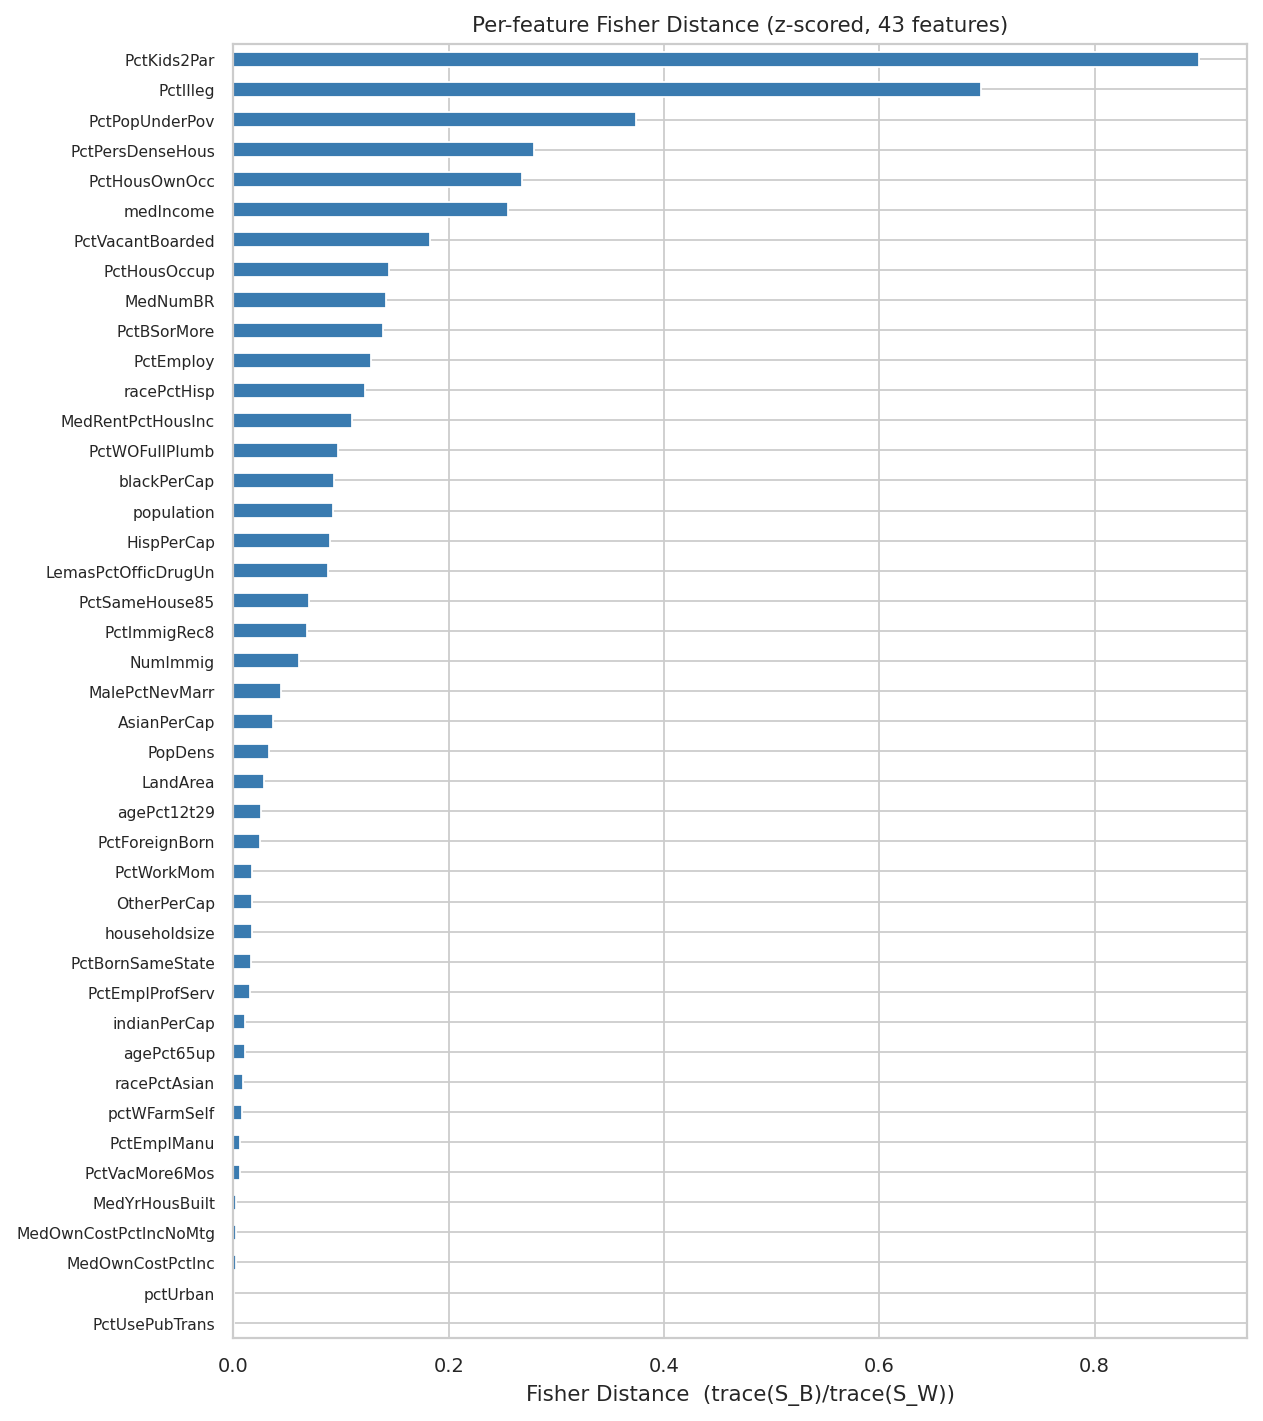
\includegraphics[width=\columnwidth]{fisher_features.png}
\caption{Z-skor normalizasyonu sonrası özellik-başına Fisher Uzaklığı, $43$ özelliğin tamamı sıralanmış halde. \texttt{PctKids2Par} ve \texttt{PctIlleg} domine eder; özelliklerin yaklaşık yarısı sıfıra yakın Fisher Uzaklığına sahiptir.}
\label{fig:fisher_feat}
\end{figure}

Elde edilen sıralama (Şekil~\ref{fig:fisher_feat}), Bölüm~\ref{sec:corr}'ün korelasyon sıralamasıyla neredeyse aynıdır; bu beklenen bir sonuçtur: tek bir z-skorlanmış özellik için hem Fisher Uzaklığı hem de mutlak sınıf korelasyonu, sınıf ortalamaları arasındaki kontrastı sınıf-içi saçılmaya göre ölçer. En üst iki özellik \texttt{PctKids2Par} ($J\!=\!0{,}90$) ve \texttt{PctIlleg} ($J\!=\!0{,}69$) olup, bunları \texttt{PctPopUnderPov} ($0{,}37$), \texttt{PctPersDenseHous} ($0{,}28$), \texttt{PctHousOwnOcc} ($0{,}27$) ve \texttt{medIncome} ($0{,}26$) izler. İki yapısal gözlem öne çıkar. İlki, ayırt edici içerik keskin biçimde yoğunlaşmıştır: \texttt{PctKids2Par} ve \texttt{PctIlleg} diğer her özelliği gölgede bırakır ve üçüncü sıradaki \texttt{PctPopUnderPov}'a doğru büyük bir düşüş vardır; onun skoru \texttt{PctIlleg}'inkinin yarısından azdır. İkincisi, $43$ özelliğin yaklaşık yarısı $0{,}03$'ün altında Fisher Uzaklığına sahiptir --- \texttt{pctUrban} ve \texttt{PctUsePubTrans} etkin biçimde sıfırdır ($J\approx 2\times 10^{-4}$); konut-maliyeti oranları \texttt{MedOwnCostPctInc} ve \texttt{MedYrHousBuilt} de öyle. Başka bir deyişle, çalışma kümesi $43$ kavramsal olarak ayrı ekseni kapsasa da, tek-özellik sınıf sinyali bunların yalnızca yaklaşık altı ila onunda yaşar. Bu yoğunlaşma, Bölüm~\ref{sec:pca}'nın temel bileşen analizini önceler: çoğu tekil eksen sınıf-bilgisiz olduğunda ve bilgili olanlar birbiriyle korelasyonlu olduğunda, çok az sayıda doğrusal kombinasyon ayrılabilirliğin neredeyse tamamını yakalamalıdır.

\section{TEMEL BİLEŞEN ANALİZİ}
\label{sec:pca}
Z-skorlanmış veriye PCA \cite{jolliffe} uygulanarak $43$ temel bileşen üretilmiştir. Başat bileşen PC1 varyansın $\%18{,}6$'sını, PC2 ise ek olarak $\%14{,}3$'ünü açıklar; ilk beş bileşen birlikte toplam varyansın yalnızca $\%53{,}4$'ünü oluşturur ve $\%80$'e ulaşmak için on altı bileşen gerekir (Şekil~\ref{fig:scree}). Bu nedenle scree eğrisi, küçük elle-seçilmiş bir özellik kümesine kıyasla çok daha düzdür: $43$ özellik kasıtlı olarak birçok zayıf-korelasyonlu kavramsal bloğu kapsadığından, varyans tek bir başat eksende toplanmak yerine birçok yöne dağılır.

\begin{figure}[!t]
\centering
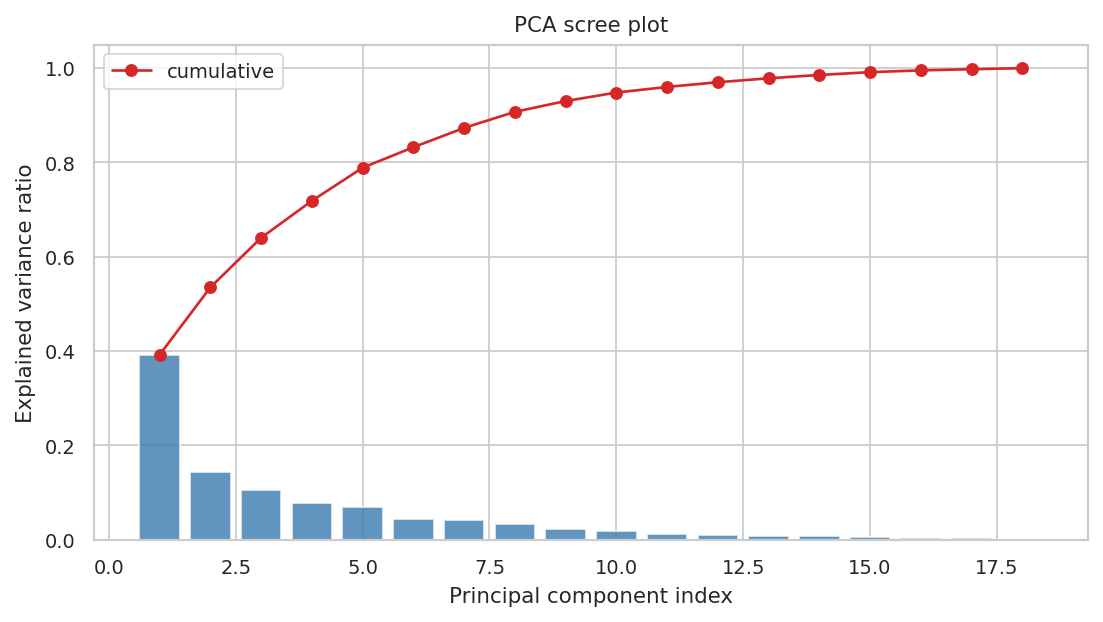
\includegraphics[width=\columnwidth]{pca_scree.png}
\caption{$43$-özellik çalışma kümesi için PCA scree grafiği. PC1 varyansın $\%18{,}6$'sını, PC2 ek $\%14{,}3$'ünü yakalar; ilk beş bileşen $\%53{,}4$'ü, $\%80$ için on altı bileşen gereklidir.}
\label{fig:scree}
\end{figure}

Her PC projeksiyonu bir özellik gibi ele alınarak Denklem~(\ref{eq:fisher})'deki Fisher Uzaklığı yeniden hesaplanmıştır (Şekil~\ref{fig:fishercmp}). PC1'in Fisher Uzaklığı $0{,}56$ olup temel bileşenler arasında açık ara en büyüğüdür; diğer her PC $0{,}07$'nin altında skor alır. Ancak kritik biçimde, PC1'in $0{,}56$'sı en iyi iki orijinal özellikten (\texttt{PctKids2Par} $0{,}90$ ve \texttt{PctIlleg} $0{,}69$) bile \emph{daha düşüktür}. Denetimsiz başat bileşen, dolayısıyla, en iyi ham özelliği basitçe tutmaktan daha kötü bir tek-eksenli sınıf ayırıcıdır; çünkü PC1 toplam varyansı maksimize etmek üzere kurulur ve ayırt edici ``avantaj--dezavantaj'' yönünü, korelasyonlu ama daha az ayırt edici varyasyonla zorunlu olarak harmanlar. Bu, Bölüm~\ref{sec:lda}'nın denetimli projeksiyonunun (LDA) temel gerekçesidir.

\begin{figure}[!t]
\centering
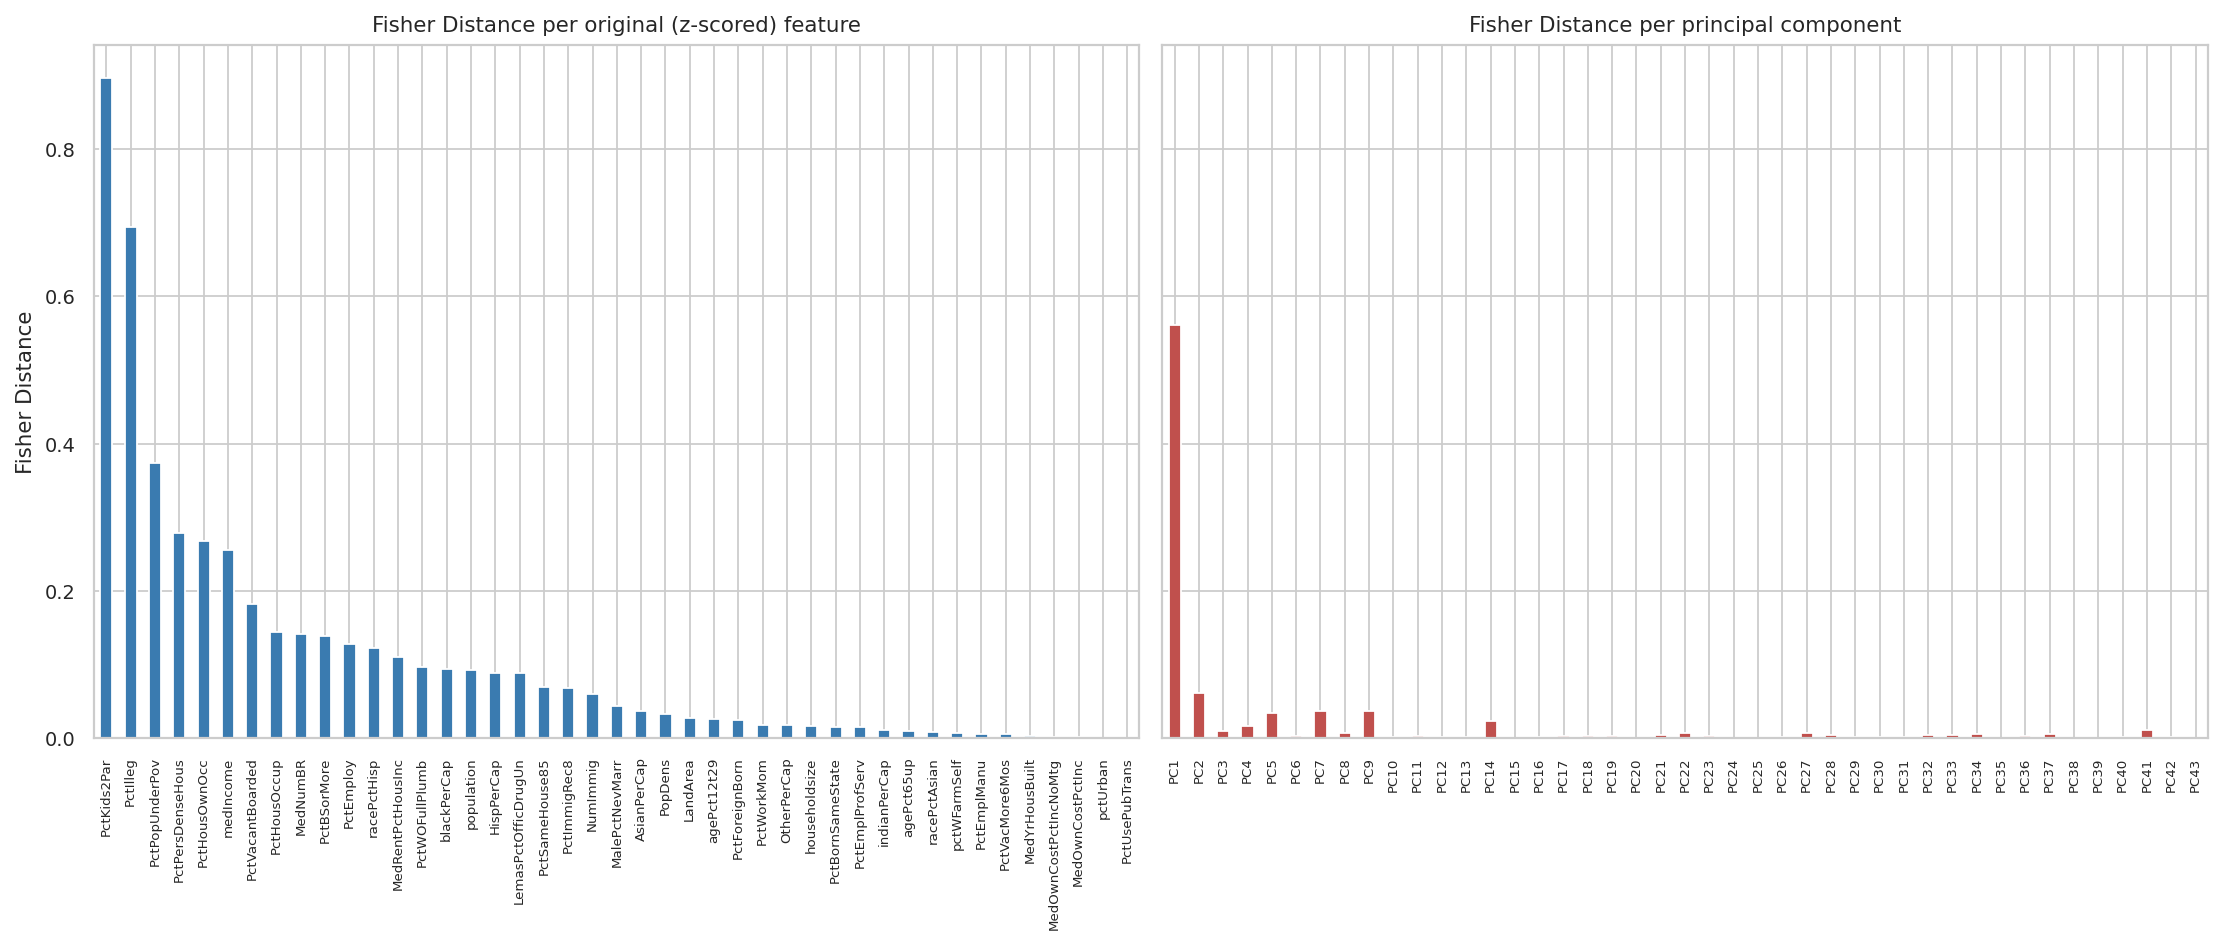
\includegraphics[width=\columnwidth]{fisher_comparison.png}
\caption{Z-skorlanmış orijinal özellik-başına (sol) ve temel bileşen-başına (sağ) Fisher Uzaklığı, ortak dikey ölçekte. Özellik-başına sinyal birkaç değişkene yayılırken, PC-başına sinyal neredeyse tamamen PC1'de yoğunlaşmıştır.}
\label{fig:fishercmp}
\end{figure}

\begin{figure}[!t]
\centering
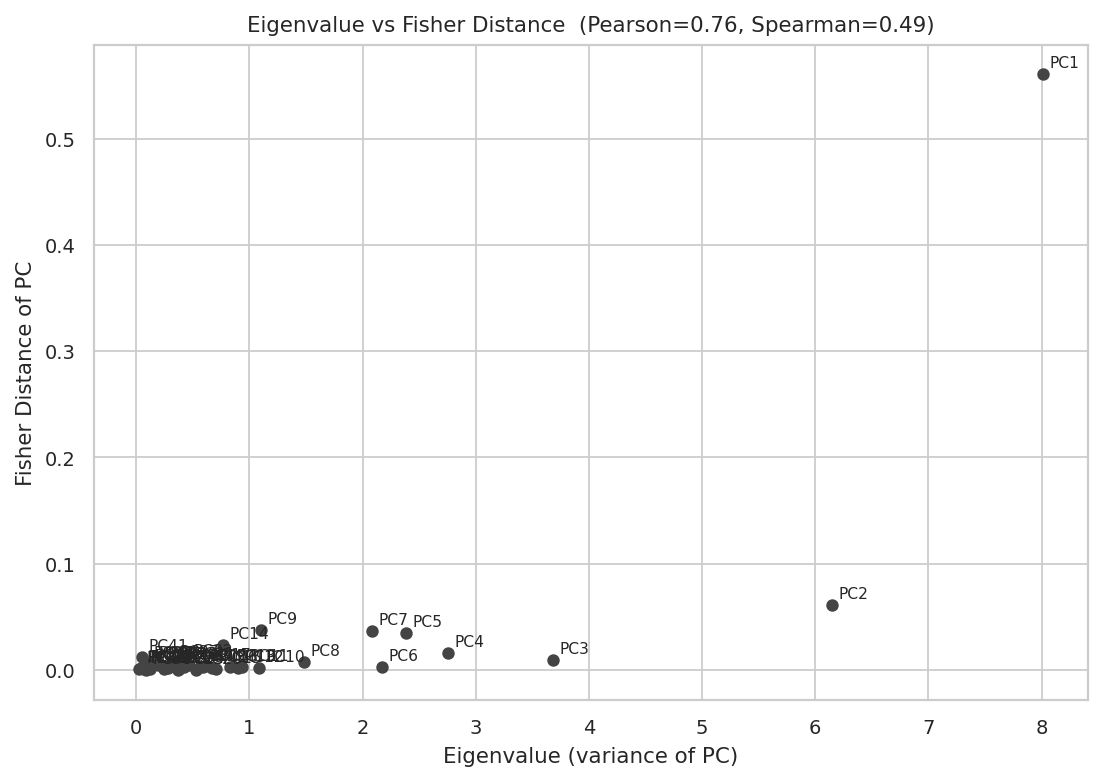
\includegraphics[width=0.95\columnwidth]{eigval_vs_fisher.png}
\caption{$43$ temel bileşen için eigenvalue'ya karşı Fisher Uzaklığı. Pearson korelasyonu $r=0{,}76$, Spearman $\rho=0{,}49$. PC2 ikinci en büyük eigenvalue'ya sahip olmasına rağmen sıfıra yakın Fisher Uzaklığı taşır.}
\label{fig:eigfisher}
\end{figure}

Bir temel bileşenin eigenvalue'su (varyansı) ile Fisher Uzaklığı arasındaki ilişki pozitif ama zayıftır ve tamamen başat bileşende yoğunlaşmıştır: Pearson korelasyonu $r=0{,}76$, Spearman sıra korelasyonu ise yalnızca $\rho=0{,}49$'dur (Şekil~\ref{fig:eigfisher}). Yüksek Pearson katsayısı, saçılımın uzak köşesinde hem en büyük eigenvalue'ya hem de açık ara en büyük Fisher Uzaklığına sahip PC1 tarafından tek başına sürüklenen bir yapay sonuçtur; PC1 çıkarıldığında eigenvalue--Fisher ilişkisi esasen kaybolur. En açık örnek \textbf{PC2}'dir: ikinci en büyük varyansı ($\%14{,}3$) taşımasına karşın Fisher Uzaklığı sıfıra yakındır ($0{,}06$); PC3 (üçüncü en büyük varyans) ise yalnızca $0{,}01$ alır. Bu yüksek-varyanslı, sınıf-ilgisiz bileşenler, PCA'nın varyansı maksimize ettiğinin, sınıf ayrılabilirliğini \emph{değil}, ders kitabı uyarısının doğrudan bir göstergesidir: PC2, suç gradyanına dik --- üç sınıfın esasen ayırt edilemez olduğu --- büyük bir topluluk-varyasyon eksenini yakalar. Yalnızca PC1 ayırt edici yönle hizalanır, o bile kusurlu biçimde. Bu, daha küçük bir özellik kümesinin düşündüreceğinden daha nüanslı bir tablodur; orada PC1 tek başına hem varyansı hem ayrılabilirliği domine etme eğilimindedir. Tam $43$-boyutlu kümede ise varyans ve ayırt edicilik, başat bileşenin ötesinde açıkça ayrışır.

\section{DÜŞÜK-BOYUTLU SINIF PROJEKSİYONLARI}
\label{sec:pcscatter}
Şekil~\ref{fig:pcscat}, temizlenmiş verinin en önemli iki ve en önemsiz iki temel bileşen üzerine projeksiyonunu, örnekler gerçek sınıf etiketlerine göre renklendirilmiş biçimde gösterir.

\begin{figure}[!t]
\centering
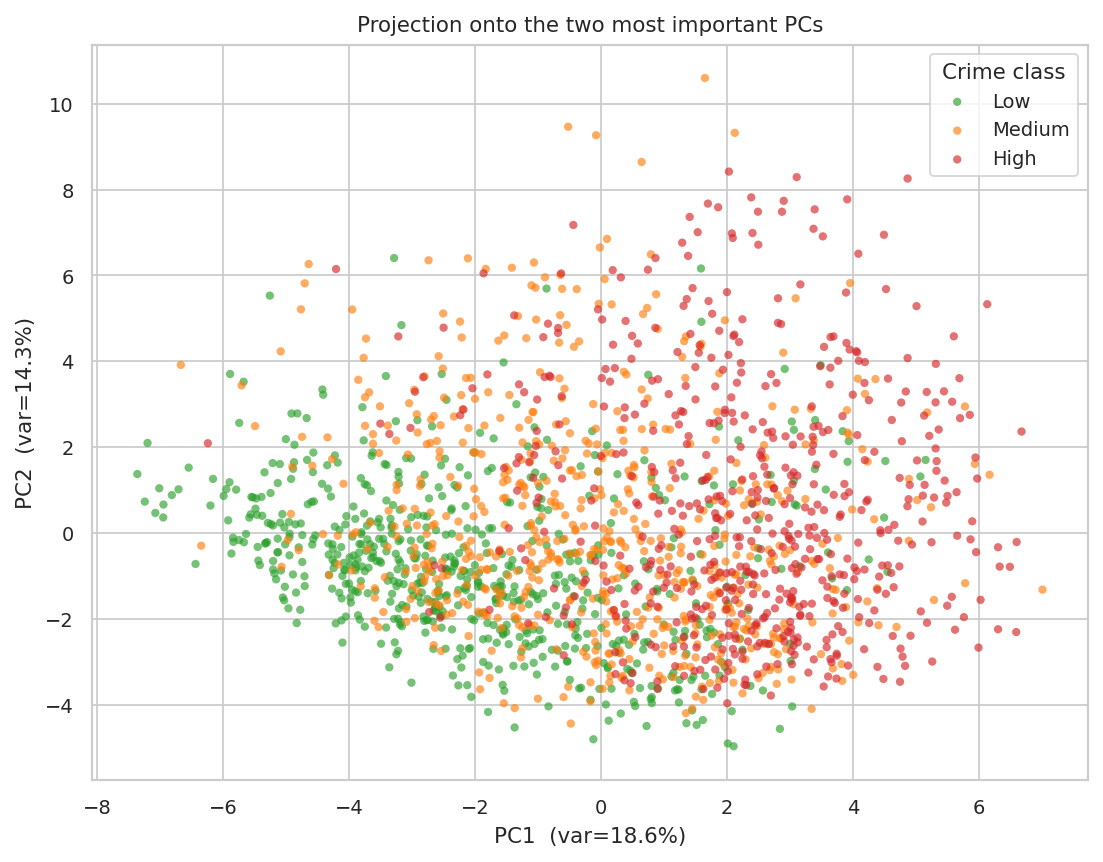
\includegraphics[width=\columnwidth]{pca_top2.png}
\\[2pt]
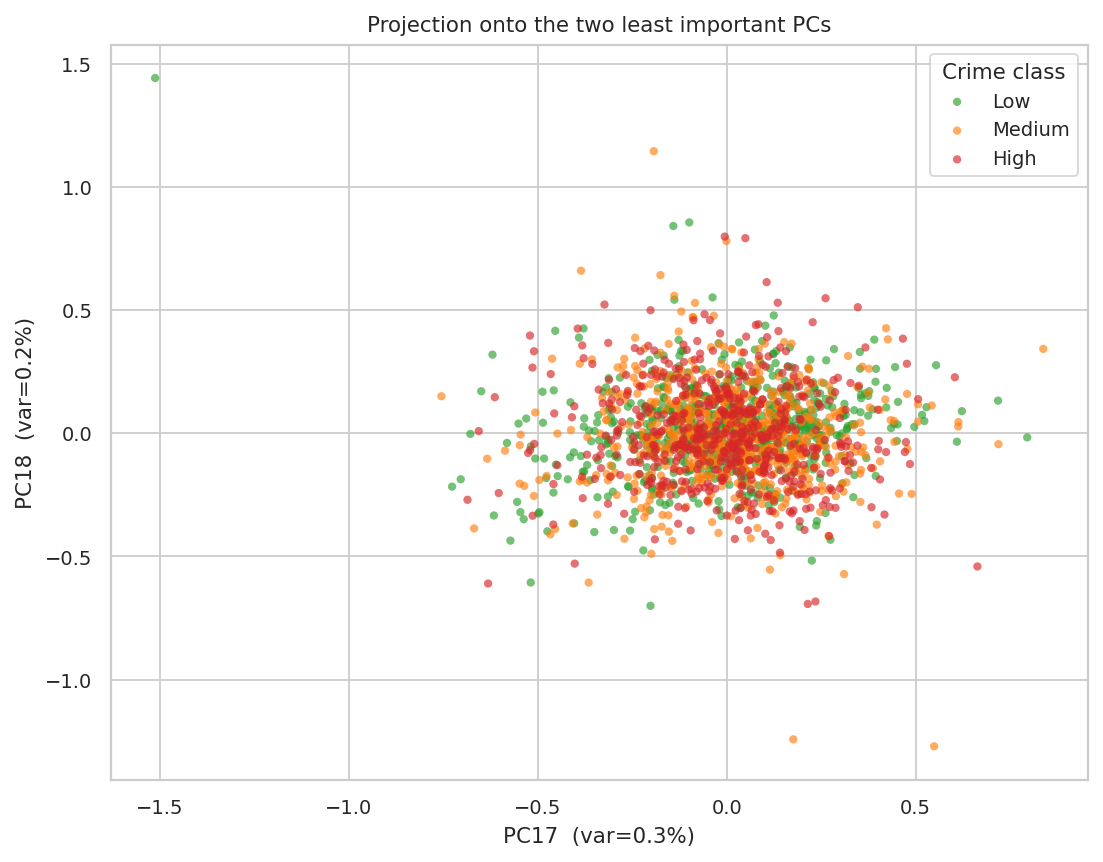
\includegraphics[width=\columnwidth]{pca_bottom2.png}
\caption{Üst: (PC1, PC2) üzerine projeksiyon. Yatay PC1 ekseni boyunca Düşük $\rightarrow$ Orta $\rightarrow$ Yüksek monoton bir sıralama belirirken, dikey PC2 ekseni hiçbir ayrım katmaz. Alt: en önemsiz iki PC (PC42, PC43) üzerine projeksiyon; hiçbir sınıf yapısı göstermez.}
\label{fig:pcscat}
\end{figure}

(PC1, PC2) grafiği, Bölüm~\ref{sec:pca}'daki ayrışmayı doğrudan görünür kılar. Yatay PC1 ekseni boyunca üç sınıf temiz, neredeyse monoton bir gradyan oluşturur: \emph{Düşük}-suç toplulukları negatif tarafta, \emph{Yüksek}-suç toplulukları pozitif tarafta yoğunlaşır ve \emph{Orta} topluluklar aradaki örtüşen bir bantta yer alır. Buna karşılık dikey PC2 ekseni boyunca üç sınıf tamamen iç içe geçmiştir: ikinci en büyük varyansı ($\%14{,}3$) taşımasına rağmen PC2 hiçbir sınıf ayrımı sağlamaz. Grafiğin tüm dikey yayılımı dolayısıyla sınıf-ilgisiz varyasyondur --- PC2'nin sıfıra yakın Fisher Uzaklığının görsel karşılığı --- ve bir topluluğu yüksek-suçlu kılan şeyin, en büyük rakip varyasyon ekseni üzerindeki konumu değil, tek PC1 ``avantaj--dezavantaj'' ekseni üzerindeki konumu olduğunu doğrular. Her biri varyansın yalnızca $\%0{,}1$'ini yakalayan en önemsiz iki bileşen (PC42, PC43) üzerine projeksiyon ise zıt uçu gösterir: üç sınıf, gürültü-benzeri artık varyans yakalayan yönler için beklendiği gibi, ayırt edilebilir hiçbir yapı olmaksızın küçük izotropik bir bulutta iç içe geçer.

\section{DOĞRUSAL AYIRMA ANALİZİ VE SINIF AYRILABİLİRLİĞİ}
\label{sec:lda}
$n_{\text{bileşen}}=2$ ile bir Doğrusal Ayırma Analizi (LDA) \cite{fisher1936} uygulanmıştır. Yapısı gereği LDA, sınıflar-arası saçılmayı sınıf-içi saçılmaya göre maksimize eder ve bu nedenle sınıf bilgisi mevcut olduğunda PCA'ya kıyasla daha sıkı sınıf-ayrılabilir bir 2-B gömme üretme eğilimindedir.

\begin{figure}[!t]
\centering
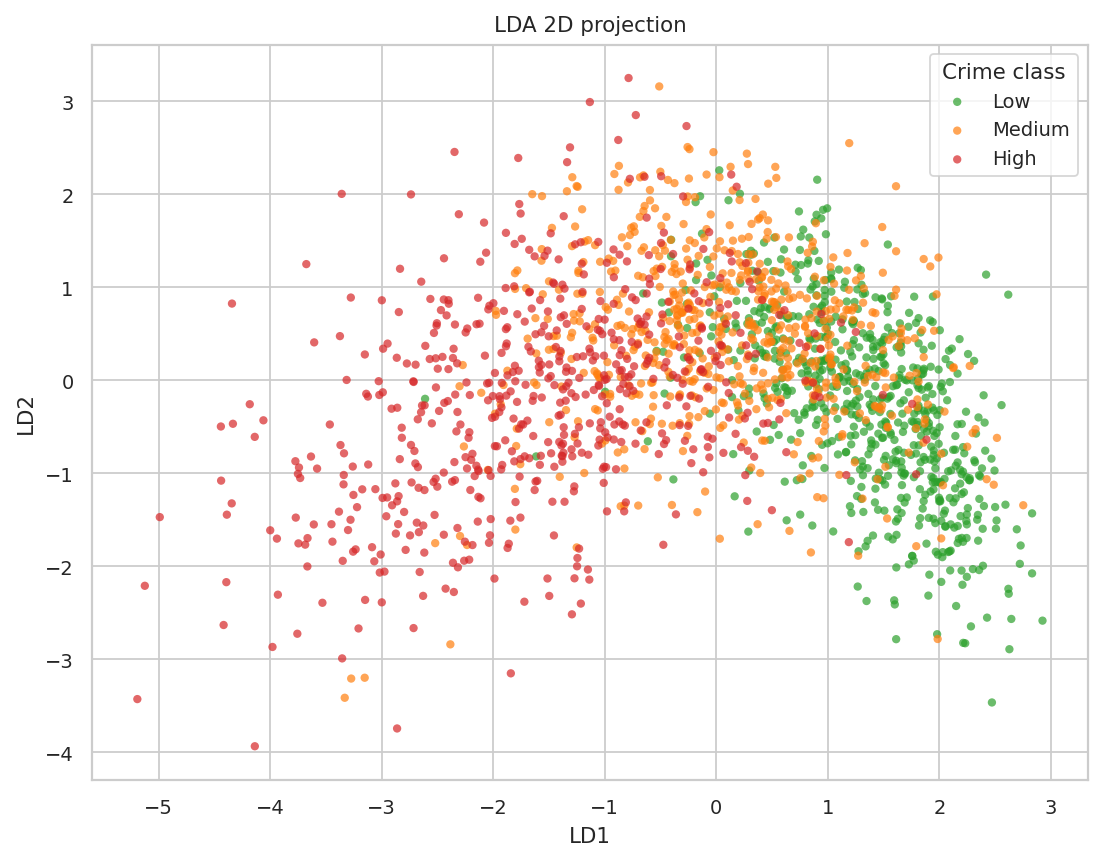
\includegraphics[width=\columnwidth]{lda_scatter.png}
\caption{LDA 2-B projeksiyonu. Üç sınıf, PCA projeksiyonuna kıyasla LD1 ekseni boyunca daha net bir sol--sağ sıralama oluşturur.}
\label{fig:lda}
\end{figure}

\begin{table}[!t]
\caption{2-B PCA ve LDA gömmelerinin nicel ayrılabilirliği. Her iki ölçüde de yüksek değer daha iyidir.}
\label{tab:sep}
\centering
\begin{tabular}{lcc}
\toprule
Ölçü & PCA (PC1,PC2) & LDA (LD1,LD2) \\
\midrule
Silüet (gerçek etiketler) & $0{,}049$ & $0{,}127$ \\
5-NN doğruluk (5-kat ÇD) & $0{,}569$ & $0{,}659$ \\
\bottomrule
\end{tabular}
\end{table}

Karşılaştırmayı nicel kılmak için 2-B gömmelerde iki ölçü hesaplanmıştır (Tablo~\ref{tab:sep}). Silüet katsayısı \cite{rousseeuw} (gerçek sınıf etiketleri bölümleme olarak kullanılarak) PCA için $0{,}049$'dan LDA için $0{,}127$'ye yükselir; bu yaklaşık $\%160$'lık ($2{,}6\times$) bir artıştır. 2-B gömme üzerinde eğitilen bir 5-NN sınıflandırıcının ortalama 5-kat çapraz-doğrulanmış doğruluğu PCA'da $\%56{,}9$'dan LDA'da $\%65{,}9$'a iyileşir; bu $+9{,}0$ yüzde puanlık bir kazançtır. Her iki ölçü de Şekil~\ref{fig:pcscat} ve \ref{fig:lda}'nın gösterdiğini doğrular: LDA, PCA'ya kıyasla belirgin biçimde daha sıkı sınıf ayrılabilirliği ortaya koyar. Önemli olarak, bu fark $43$-özellik kümesinde, düşük-boyutlu bir analizin düşündüreceğinden \emph{daha geniştir} ve nedeni doğrudan Bölüm~\ref{sec:pca}'dan gelir. PCA gömmesi iki ekseninden birini (PC2) mevcut en büyük varyans yönüne harcamak zorundadır; Bölüm~\ref{sec:pca} bu yönün sınıf-ilgisiz olduğunu göstermiştir; yalnızca PC1 sınıf sinyali taşır, dolayısıyla PCA etkin biçimde tek kullanışlı ayırt edici eksene sahiptir. Denetimli olan LDA ise \emph{her iki} eksenini de sınıflar-arası saçılmayı sınıf-içine göre maksimize edecek şekilde yönlendirir ve böylece zengin $43$-boyutlu özellik uzayından çok daha verimli yararlanır. Kısacası, PCA 2-B bütçesinin yarısını sınıf-ilgisiz varyansa harcarken LDA harcamaz; ölçü farkı tam olarak bu farkı niceler.

\section{DENETİMSİZ KÜME YAPISI}
\label{sec:cluster}
Dört algoritma iki farklı girdiyle uygulanmıştır. K-Means ($k\!=\!3$) \cite{lloyd} ve DBSCAN ($\varepsilon\!=\!0{,}5$, $\mathrm{minPts}\!=\!10$) \cite{ester} 2-B PCA projeksiyonu (PC1, PC2) üzerinde çalışır. t-SNE (perplexity $30$, PCA başlatma) \cite{vandermaaten} ve $12\times 12$ Öz-Düzenleyici Harita \cite{kohonen}, \cite{minisom} ise tam $43$-boyutlu z-skorlanmış veriye uygulanır.

\begin{figure}[!t]
\centering
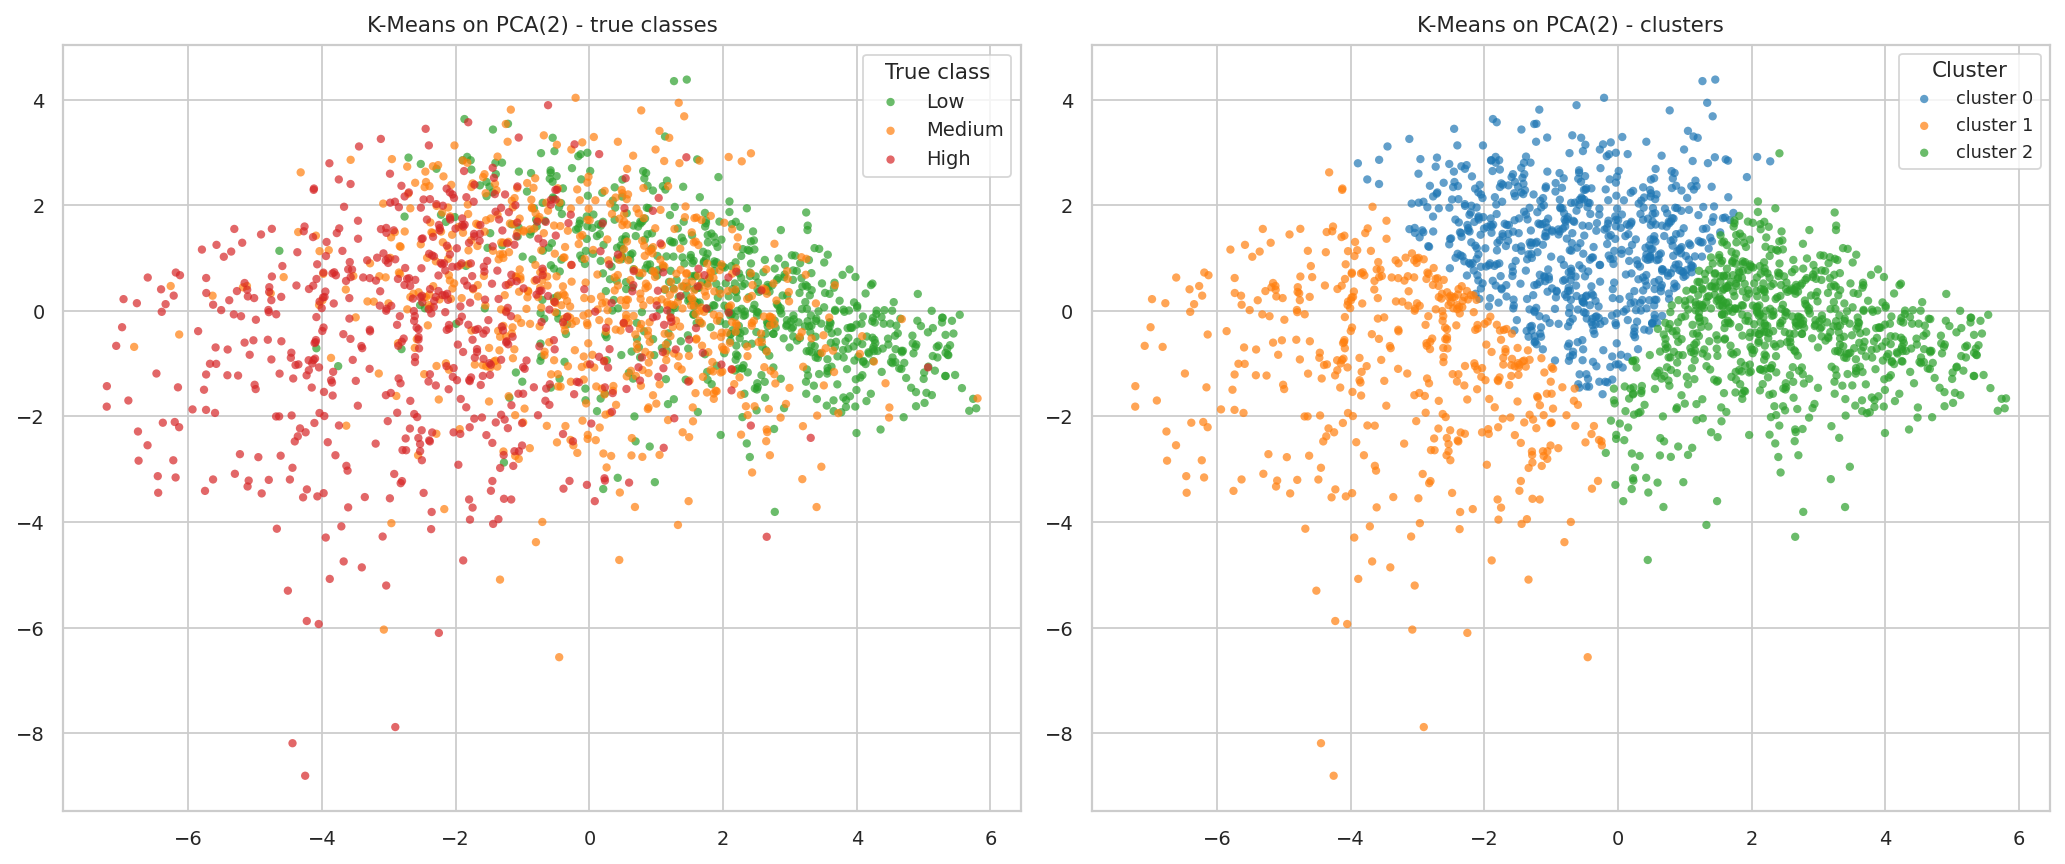
\includegraphics[width=\columnwidth]{cluster_kmeans.png}
\caption{(PC1, PC2) projeksiyonu üzerinde K-Means ($k=3$). Sol: gerçek sınıflar; sağ: atanan kümeler.}
\label{fig:kmeans}
\end{figure}

\begin{figure}[!t]
\centering
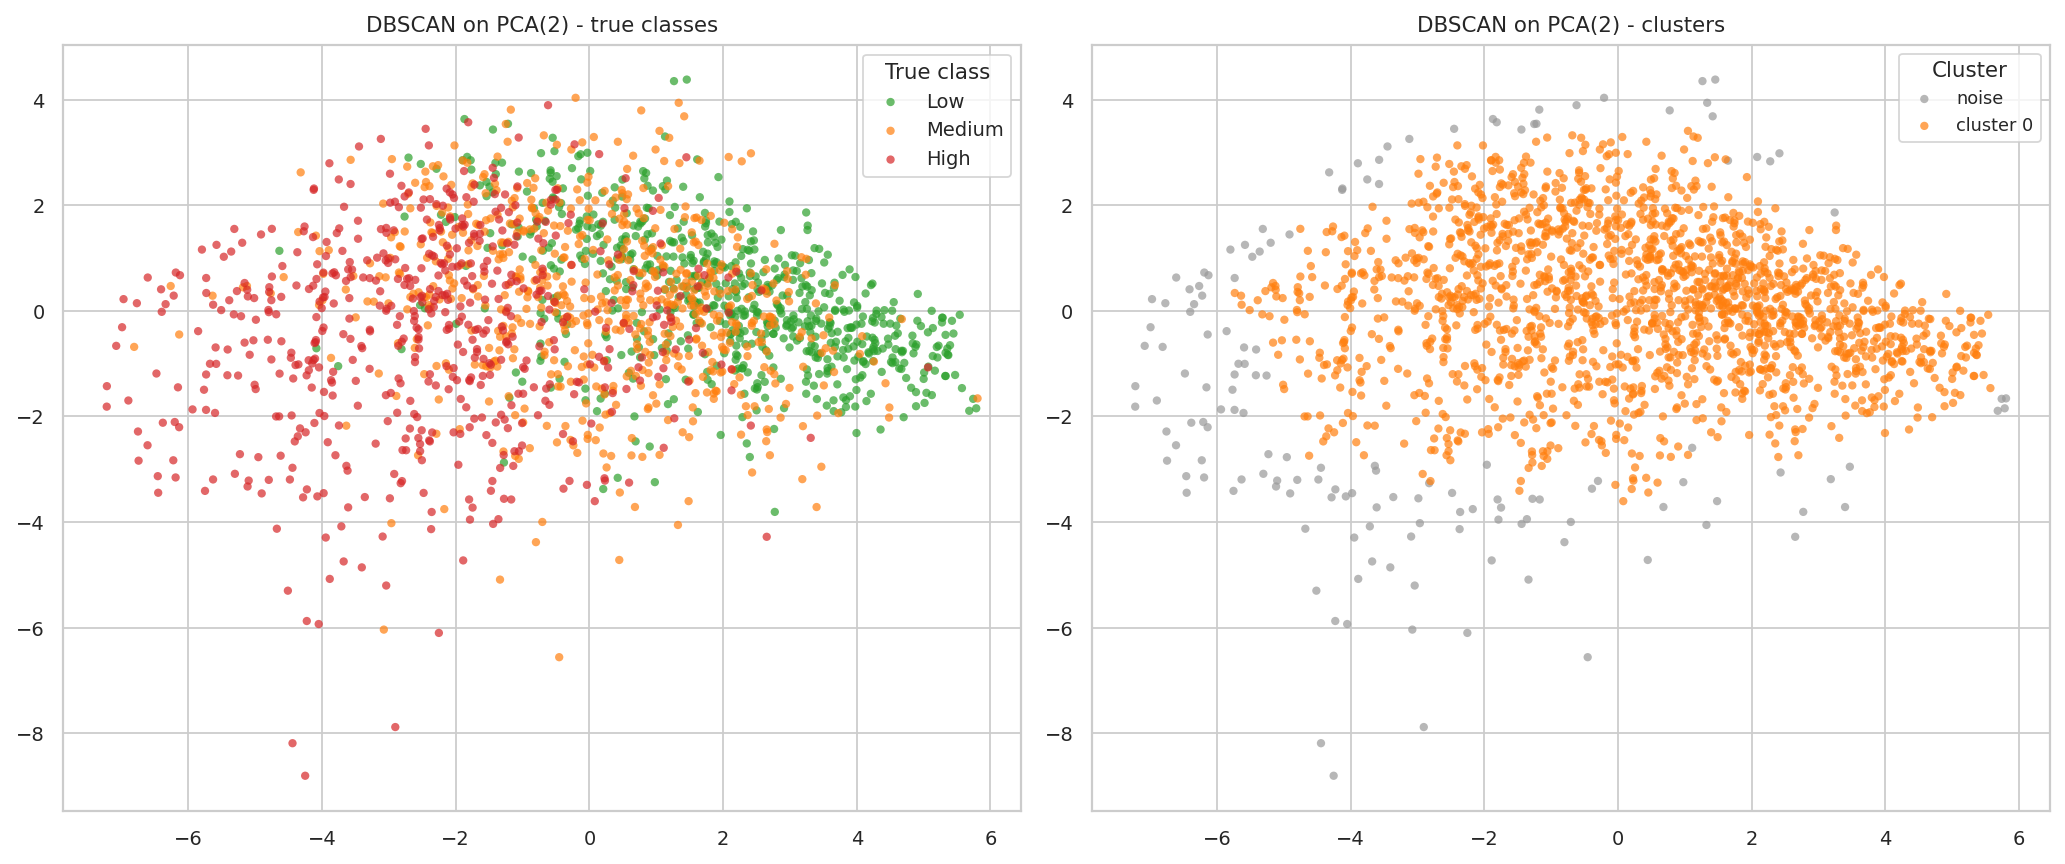
\includegraphics[width=\columnwidth]{cluster_dbscan.png}
\caption{(PC1, PC2) üzerinde DBSCAN ($\varepsilon=0{,}5$, $\mathrm{minPts}=10$). Verinin büyük kısmı tek bir baskın yoğun kümede toplanır (artı birkaç küçük kenar kümesi), $233$ örnek ($\%12{,}3$) gürültü olarak işaretlenir.}
\label{fig:dbscan}
\end{figure}

\begin{figure}[!t]
\centering
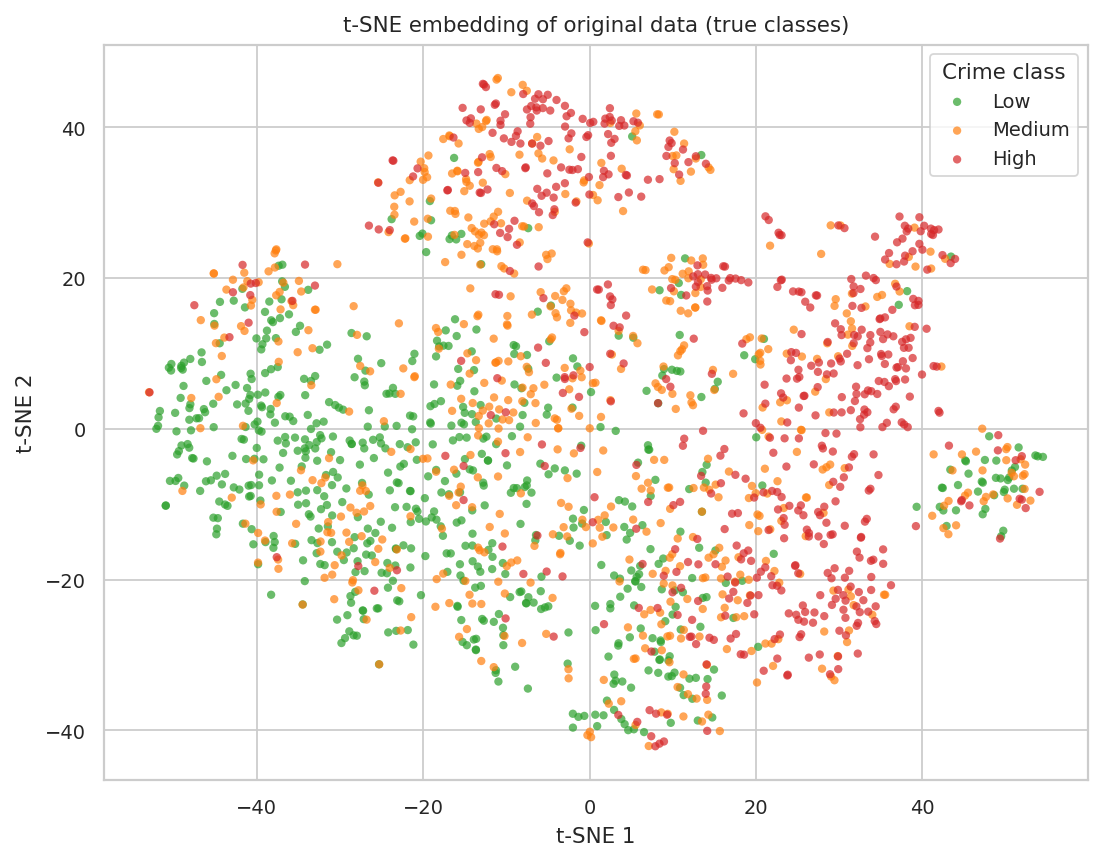
\includegraphics[width=\columnwidth]{cluster_tsne.png}
\caption{Tam $43$-boyutlu z-skorlanmış verinin, gerçek sınıfa göre renklendirilmiş t-SNE gömmesi. Gömme boyunca sürekli bir gradyan görünür.}
\label{fig:tsne}
\end{figure}

\begin{figure}[!t]
\centering
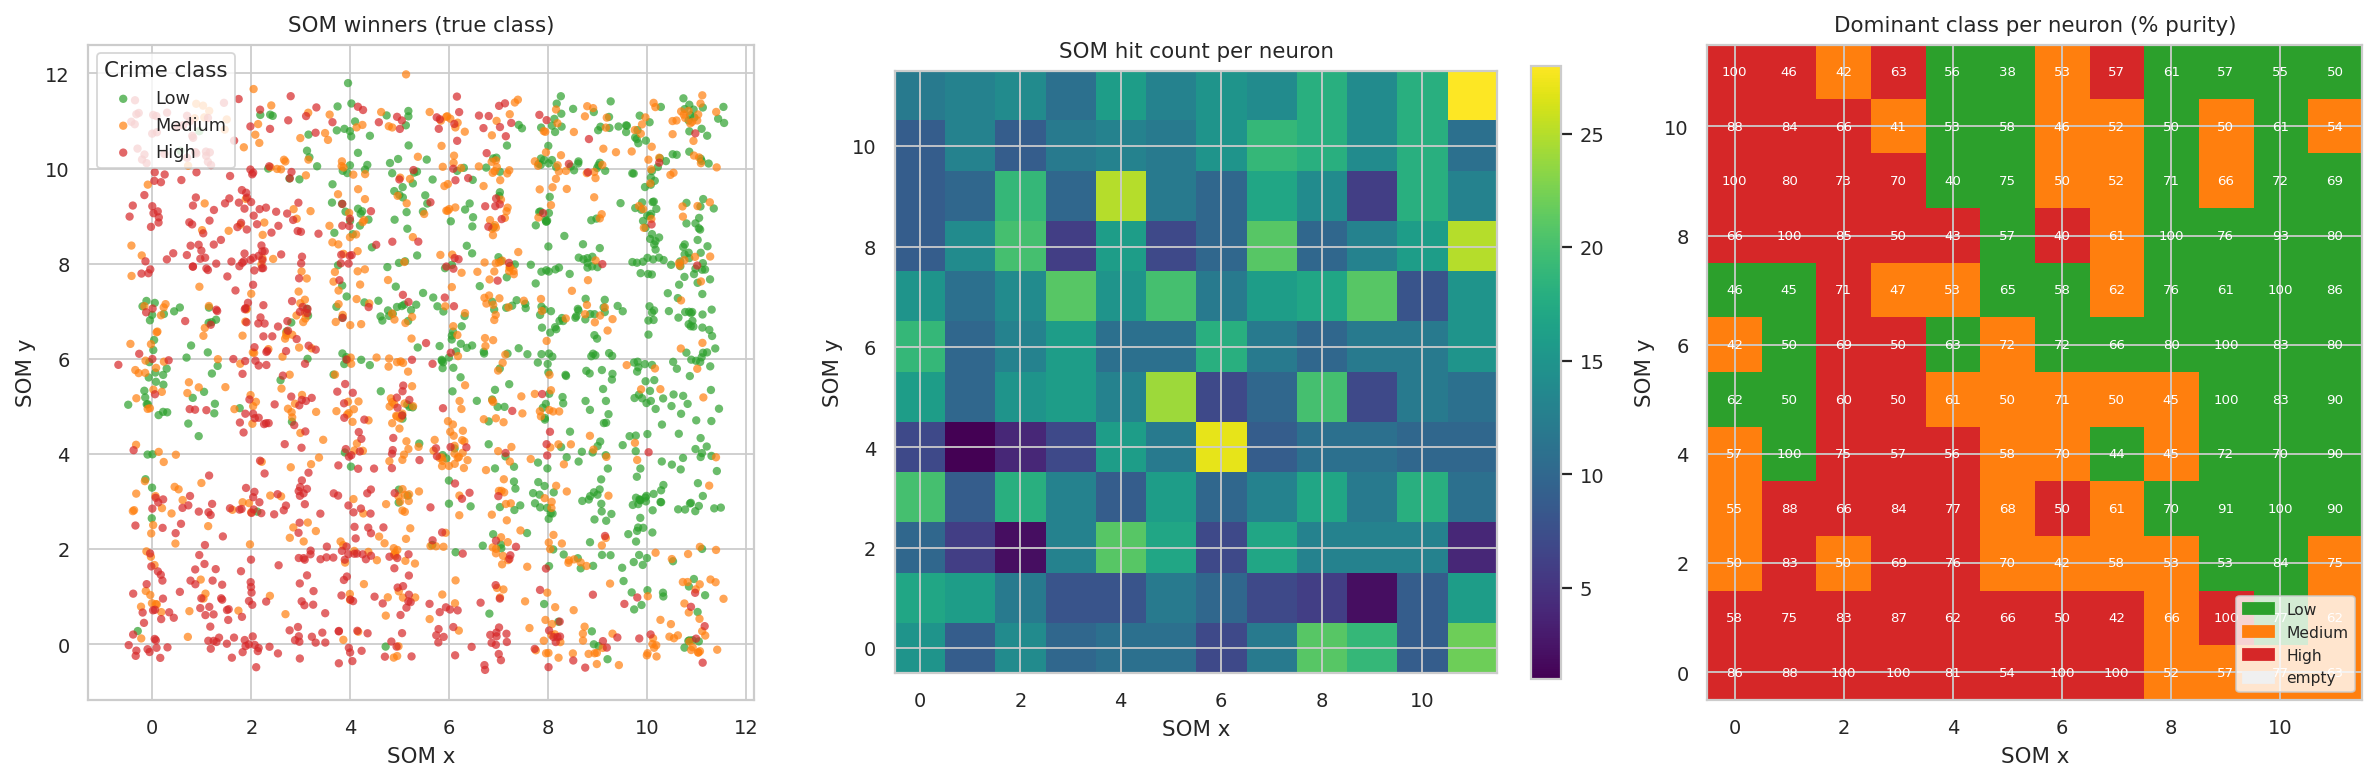
\includegraphics[width=\columnwidth]{cluster_som.png}
\caption{Orijinal z-skorlanmış veride eğitilmiş $12\times 12$ MiniSom. Sol: kazananların gerçek sınıfa göre saçılımı (görünürlük için titreştirilmiş). Orta: nöron-başına vuruş-sayısı ısı haritası. Sağ: nöron-başına baskın sınıf ve hücre-başına saflık (metin etiketleri, $\%$ olarak); boş olmayan hücrelerin ortalama saflığı $\%67{,}5$'tir.}
\label{fig:som}
\end{figure}

\begin{table}[!t]
\caption{Küme atamaları ile gerçek sınıf etiketleri arasındaki Düzeltilmiş Rand İndeksi (ARI) \cite{hubert} ve Normalize Karşılıklı Bilgi (NMI).}
\label{tab:clust}
\centering
\begin{tabular}{lcc}
\toprule
Yöntem (girdi) & ARI & NMI \\
\midrule
K-Means, $k=3$ (PCA-2B)  & $0{,}142$ & $0{,}147$ \\
DBSCAN ($\varepsilon=0{,}5$) (PCA-2B) & $0{,}018$ & $0{,}039$ \\
\bottomrule
\end{tabular}
\end{table}

\paragraph{K-Means} (PC1, PC2) düzleminde, sınırları PC1 boyunca kabaca dikey kesimler olan üç küme bulur; bu Bölüm~\ref{sec:pcscatter}'deki gradyanı yansıtır. İki girdi ekseninden yalnızca PC1 sınıf sinyali taşıdığından, onun boyunca bölümleme gerçek etiketlerle bir miktar uyum verir (ARI $=0{,}14$, NMI $=0{,}15$); ancak bu uyum, küçük-özellikli bir analizin vereceğinden zayıftır. Nedeni Bölüm~\ref{sec:pca}--\ref{sec:lda}'da saptanan aynı ayrışmadır: K-Means PC1 ve PC2'yi izotropik biçimde ele alır; oysa PC2 (varyansın $\%14{,}3$'ü) sınıf-ilgisizdir; dolayısıyla bölümleme çabasının önemli bir kısmı toplulukları suçla ilgisiz bir yön boyunca ayırmaya harcanır. PCA düzleminde denetimsiz kümeleme, böylece PCA'nın kendi zayıflığını miras alır.

\paragraph{DBSCAN} esasen başarısız olur: $\varepsilon=0{,}5$, $\mathrm{minPts}=10$ ile tek bir baskın yoğun küme, birkaç küçük kenar kümesi ve $233$ gürültü noktası ($\%12{,}3$) üretir; ARI yalnızca $0{,}018$'dir. Veri, iyi-ayrılmış yoğunluk modları yerine tek bir sürekli ``sosyoekonomik gradyan'' oluşturduğundan, yoğunluk-tabanlı kümeleme üç sınıfı geri kazanamaz; DBSCAN, bu veri setinin sınıf yapısının modal değil gradyan-benzeri olduğunu açığa çıkarır.

\paragraph{t-SNE} tam $43$-boyutlu veride, üç sınıfın ayrık adalar yerine sürekli bir gradyan oluşturduğu (\emph{Düşük} bir uçta, \emph{Yüksek} diğer uçta) tek, yumuşak değişen bir nokta bulutu üretir. Bu, sınıfların büyük ölçüde tek-boyutlu bir sosyoekonomik süreklilik üzerindeki konumla tanımlandığı --- kompakt modal kümelerle değil --- görüşünü pekiştirir; aynı sonuca PCA, DBSCAN ve SOM bağımsız olarak ulaşır.

\paragraph{SOM} $12\times 12$ MiniSom ızgarası (Şekil~\ref{fig:som}) en sınıf-organize doğrusal-olmayan görünümü sağlar. Vuruş-sayısı ısı haritası (orta panel), SOM'un kapasiteyi ızgaraya birkaç biraz daha yoğun merkezle düzgünce dağıttığını gösterir. Baskın-sınıf paneli (sağ), latis üzerinde bir gradyan boyunca dizilmiş bitişik Düşük, Orta ve Yüksek sınıf bölgelerini, bazı hücreler $\geq \%90$ saflığa ulaşacak şekilde ortaya koyar. Boş olmayan hücrelerin ortalama nöron-başına saflığı $\%67{,}5$ olup, (neredeyse-tekdüze) sınıf dağılımı altında şanstan beklenen $\approx \%35$'in çok üstündedir. SOM, böylece, orijinal $43$-boyutlu özellik uzayında t-SNE haritasında görülen aynı gradyan-benzeri organizasyonu doğrular.

\section{BAŞAT ÖNGÖRÜCÜNÜN ANLAMLILIĞI}
\label{sec:hypothesis}
Hipotez testi için \texttt{PctKids2Par} özelliği (iki-ebeveynli hanelerde yaşayan çocukların yüzdesi) seçilmiştir; çünkü en büyük Fisher Uzaklığına ve sınıf etiketiyle en büyük mutlak korelasyona sahiptir (Bölüm~\ref{sec:corr}--\ref{sec:fisher}). Test edilecek hipotez, bu özelliğin ortalamasının \emph{Düşük} ve \emph{Yüksek} suç sınıfları arasında eşitliğidir:
\begin{align*}
H_0:\ \mu_{\text{Düşük}} = \mu_{\text{Yüksek}}, \qquad
H_1:\ \mu_{\text{Düşük}} \neq \mu_{\text{Yüksek}}.
\end{align*}
Her sınıftan $n=36$ ve $n=64$ büyüklüğünde iki bağımsız rastgele örnek (yerine koymadan) çekilmiş ve iki-yönlü Welch t-testi \cite{welch} (eşit varyans varsaymayan) uygulanmıştır. Sonuçlar Tablo~\ref{tab:ttest}'de özetlenmiştir.

\begin{table}[!t]
\caption{Düşük ve Yüksek suç sınıfları arasında \texttt{PctKids2Par} üzerinde Welch t-testi sonuçları.}
\label{tab:ttest}
\centering
\begin{tabular}{lccc}
\toprule
Sınıf başına $n$ & $\bar x_{\text{Düşük}}$ ($\pm$ s.s.) & $\bar x_{\text{Yüksek}}$ ($\pm$ s.s.) & $t$ \ ($p$-değeri) \\
\midrule
$36$ & $0{,}759\pm 0{,}130$ & $0{,}463\pm 0{,}147$ & $9{,}01$ \ ($2{,}8\!\times\!10^{-13}$) \\
$64$ & $0{,}792\pm 0{,}112$ & $0{,}444\pm 0{,}188$ & $12{,}73$ \ ($7{,}3\!\times\!10^{-23}$) \\
tümü & $-$              & $-$              & $39{,}28$ \ ($\approx 10^{-207}$) \\
\bottomrule
\end{tabular}
\end{table}

Üç durumun tümünde ($36$, $64$ büyüklüğünde örnekler ve tam sınıflar) $p$-değeri, $\alpha\in\{0{,}05, 0{,}01, 0{,}001\}$ gibi herhangi bir geleneksel anlamlılık düzeyinden onlarca büyüklük mertebesi daha küçüktür. Eşit ortalama sıfır hipotezi, dolayısıyla $H_1$ lehine ezici kanıtla reddedilir: \texttt{PctKids2Par}, Düşük-suç topluluklarında Yüksek-suç topluluklarına göre ortalamada belirgin biçimde daha yüksektir (normalize ölçekte yaklaşık $0{,}79$'a karşı $0{,}45$; $[0,1]$ ölçeğinde $\approx 0{,}33$'lük bir kayma). Beklendiği gibi, örnek büyüklüğünü $36$'dan $64$'e çıkarmak örnek ortalamalarını neredeyse değiştirmezken $|t|$'yi $9{,}01$'den $12{,}73$'e yükseltir; bu, aynı etki büyüklüğü için daha büyük örneğin daha yüksek istatistiksel gücünü gösterir. Tam-sınıf $t=39{,}28$ değeri bu eğilimi mevcut verinin sınırına taşır.

\section{SONUÇ}
\label{sec:conclusion}
Bu çalışma, UCI Communities and Crime veri setine eksiksiz bir keşifsel ve istatistiksel analiz boru hattı uygulamıştır. Etiket-kör, hiyerarşik-kümeleme tabanlı bir özellik seçimi $122$ öngörücüyü redundant olmayan $43$ özelliklik bir çalışma kümesine indirgemiş ve sürekli şiddet-suç oranı üç sınıfa ayrıştırılmıştır. Şu tutarlı tablo ortaya çıkar. İlk olarak, aile-yapısı ve sosyoekonomik temsilciler (\texttt{PctKids2Par}, \texttt{PctIlleg}, \texttt{PctPopUnderPov}, \texttt{PctPersDenseHous}, \texttt{PctHousOwnOcc}, \texttt{medIncome}) en güçlü tekil sınıf sinyalini taşır; bu hem Pearson hem Spearman korelasyonu hem de özellik-başına Fisher Uzaklığı tarafından bağımsız olarak doğrulanır (Spearman--Pearson sıra uyumu $0{,}97$); veri-güdümlü küme ayrıca aşırı kalabalıklaşmayı (\texttt{PctPersDenseHous}) elle-seçilmiş bir kümenin gözden kaçırabileceği bir üst korelasyon olarak su yüzüne çıkarır; buna karşılık \texttt{pctUrban}, \texttt{agePct65up} ve \texttt{LandArea} gibi demografik ve coğrafi değişkenler esasen sınıf-bilgisizdir. İkincisi, ayırt edici içerik çok az yönde yoğunlaşmıştır ama artık tek bir başat yönde değil: PC1 varyansın yalnızca $\%18{,}6$'sını açıklar ve $0{,}56$'lık bir Fisher Uzaklığı elde eder --- bu, en iyi iki ham özellikten bile düşüktür --- ikinci en büyük varyans bileşeni PC2 ($\%14{,}3$) ise sınıf-ilgisizdir (Fisher $0{,}06$). Eigenvalue ve Fisher Uzaklığı, dolayısıyla, yalnızca zayıf biçimde ilişkilidir (tamamen PC1 tarafından sürüklenen $r=0{,}76$, $\rho=0{,}49$): yüksek varyans yüksek ayırt ediciliği gerektirmez; bu nokta PC2 tarafından çarpıcı biçimde gösterilir. Üçüncüsü, LDA 2-B gömmesi sınıf ayrılabilirliğini ortaya koymada PCA 2-B gömmesini hem görsel hem nicel olarak açıkça geçer (silüet $0{,}127$'ye karşı $0{,}049$; 5-NN ÇD doğruluğu $\%65{,}9$'a karşı $\%56{,}9$); bunun nedeni tam olarak PCA'nın iki ekseninden birini sınıf-ilgisiz varyansa harcamak zorunda olması, denetimli LDA'nın ise olmamasıdır. Dördüncüsü, denetimsiz kümeleme sınıf yapısının modal değil gradyan-benzeri olduğunu ortaya koyar: PCA düzleminde K-Means yalnızca mütevazı uyum elde eder (ARI $0{,}14$), DBSCAN $233$ gürültü noktasıyla tek baskın kümeye çöker (ARI $0{,}02$) ve hem t-SNE hem SOM, üç sınıfın yumuşakça birbirine geçtiği sürekli bir manifold üretir; yine de SOM, şans düzeyinin çok üstünde, $\%67{,}5$'lik bir ortalama nöron-başına sınıf saflığı elde eder. Son olarak, \texttt{PctKids2Par} üzerinde bir Welch t-testi, eşit sınıf ortalamaları sıfır hipotezini hem $n=36$ ($t=9{,}01$) hem $n=64$ ($t=12{,}73$) için aşırı anlamlılıkla reddederek önceki bölümlerin betimsel kanıtını biçimsel olarak doğrular.

Genel olarak, veri seti üç iyi-ayrılmış küme olarak değil, şiddet suçunun monotonik biçimde yükseldiği tek-boyutlu bir sosyoekonomik süreklilik olarak en iyi şekilde anlaşılır. Bu, denetimli bir doğrusal yöntemin (LDA) denetimsiz PCA projeksiyonunu neden geçtiğini, yoğunluk-tabanlı kümelemenin neden başarısız olduğunu ve en güçlü tekil öngörücülerin neden salt demografik değil aile-yapısı ve yoksunluk göstergeleri olduğunu açıklar. Veri-güdümlü $43$-özellik seçimi, hem elle düzenlemenin sübjektifliğini ortadan kaldırır hem de --- PCA varyansı ile sınıf ayrılabilirliği arasındaki ayrışma ve aşırı kalabalıklaşmanın rolü gibi --- daha küçük, elle-seçilmiş bir çalışma kümesinin gizleyeceği yapıyı açığa çıkarır.

\appendix
\section{A}
Tüm analiz boru hattını uygulayan Jupyter not defteri (\texttt{Crime\_Analysis.ipynb}) ve üretilen tüm şekiller bu raporla birlikte sunulmaktadır. Orijinal veri seti UCI Makine Öğrenmesi Deposundan herkese açık olarak temin edilebilir \cite{uciccrime}.

\begin{thebibliography}{99}
\bibitem{uciccrime}
M.~Redmond, ``Communities and Crime,'' UCI Machine Learning Repository, 2002, doi: 10.24432/C53W3X. [Çevrimiçi]. Erişim: \url{https://doi.org/10.24432/C53W3X}
\bibitem{redmondbaveja}
M.~A.~Redmond ve A.~Baveja, ``A data-driven software tool for enabling cooperative information sharing among police departments,'' \emph{European Journal of Operational Research}, c.~141, no.~3, s.~660--678, 2002.
\bibitem{shawmckay}
C.~R.~Shaw ve H.~D.~McKay, \emph{Juvenile Delinquency and Urban Areas}. Chicago, IL, ABD: Univ. of Chicago Press, 1942.
\bibitem{sampson}
R.~J.~Sampson, S.~W.~Raudenbush, ve F.~Earls, ``Neighborhoods and violent crime: A multilevel study of collective efficacy,'' \emph{Science}, c.~277, no.~5328, s.~918--924, 1997.
\bibitem{hastie}
T.~Hastie, R.~Tibshirani, ve J.~Friedman, \emph{The Elements of Statistical Learning}, 2.~baskı. New York, NY, ABD: Springer, 2009.
\bibitem{pedregosa}
F.~Pedregosa \emph{ve diğ.}, ``Scikit-learn: Machine Learning in Python,'' \emph{Journal of Machine Learning Research}, c.~12, s.~2825--2830, 2011.
\bibitem{liu2008isolation}
F.~T.~Liu, K.~M.~Ting, ve Z.-H.~Zhou, ``Isolation Forest,'' \emph{Proc.\ 8th IEEE Int.\ Conf.\ on Data Mining (ICDM)}, 2008, s.~413--422.
\bibitem{fisher1936}
R.~A.~Fisher, ``The use of multiple measurements in taxonomic problems,'' \emph{Annals of Eugenics}, c.~7, no.~2, s.~179--188, 1936.
\bibitem{jolliffe}
I.~T.~Jolliffe, \emph{Principal Component Analysis}, 2.~baskı. New York, NY, ABD: Springer, 2002.
\bibitem{rousseeuw}
P.~J.~Rousseeuw, ``Silhouettes: A graphical aid to the interpretation and validation of cluster analysis,'' \emph{Journal of Computational and Applied Mathematics}, c.~20, s.~53--65, 1987.
\bibitem{lloyd}
S.~P.~Lloyd, ``Least squares quantization in PCM,'' \emph{IEEE Transactions on Information Theory}, c.~28, no.~2, s.~129--137, 1982.
\bibitem{ester}
M.~Ester, H.-P.~Kriegel, J.~Sander, ve X.~Xu, ``A density-based algorithm for discovering clusters in large spatial databases with noise,'' \emph{Proc.\ 2nd Int.\ Conf.\ Knowledge Discovery and Data Mining (KDD)}, 1996, s.~226--231.
\bibitem{vandermaaten}
L.~van der Maaten ve G.~Hinton, ``Visualizing data using t-SNE,'' \emph{Journal of Machine Learning Research}, c.~9, s.~2579--2605, 2008.
\bibitem{kohonen}
T.~Kohonen, ``The self-organizing map,'' \emph{Proceedings of the IEEE}, c.~78, no.~9, s.~1464--1480, 1990.
\bibitem{minisom}
G.~Vettigli, ``MiniSom: minimalistic and NumPy-based implementation of the Self Organizing Map,'' 2018. [Çevrimiçi]. Erişim: \url{https://github.com/JustGlowing/minisom}
\bibitem{hubert}
L.~Hubert ve P.~Arabie, ``Comparing partitions,'' \emph{Journal of Classification}, c.~2, no.~1, s.~193--218, 1985.
\bibitem{welch}
B.~L.~Welch, ``The generalization of `Student's' problem when several different population variances are involved,'' \emph{Biometrika}, c.~34, no.~1/2, s.~28--35, 1947.
\end{thebibliography}

\begin{IEEEbiography}[{
\includegraphics[width=1in,height=1.25in,clip,keepaspectratio]{serkan_vek.jpg}}]{Serkan Eren}
B.Sc.\ derecesini 2023 yılında Gebze Teknik Üniversitesi Elektronik Mühendisliği Bölümü'nden almış olup, hâlihazırda aynı üniversitede Yapay Zekâ alanında M.Sc.\ programını sürdürmektedir. FEV Türkiye bünyesinde Otomotiv Yazılım Mühendisi olarak görev yapmakta; Python tabanlı otomasyon, DevOps boru hatları ve gömülü yazılım entegrasyonu konularında çalışmalar yürütmektedir. Mesleki ilgi alanları derin öğrenme, akıllı sistemler için yazılım mühendisliği ve otomasyon ile doğal dil işleme için veri-güdümlü uygulama geliştirmedir.
\end{IEEEbiography}

\EOD
\end{document}
